\chapter{The finite element code Legolas} \label{ch: Legolas}

\graphicspath{{04-legolas/figures/}}

\begin{chapterquote}[Stephen Hawking][A Brief History of Time][]
  Any physical theory is always provisional, in the sense that it is only a hypothesis; you can never prove it. No matter how many times the results of experiments agree with some theory, you can never be sure that the next time the result will not contradict the theory.
\end{chapterquote}

\usespublishedwork{
  Most of this Chapter was published in ``Legolas: a novel tool for magnetohydrodynamic spectroscopy'', 2020, \apjs,
  251, 25 \citep{claes2020_legolas}. N. Claes developed {\legolas} in close collaboration with J. De Jonghe, generated the data and figures and wrote a first draft of the manuscript; J. De Jonghe revised and extended the manuscript. R. Keppens contributed to the revision of the paper.
}

In the previous Chapter we looked at wave modes and growth rates in simple planar, uniform configurations. Naturally, the next step would be adding a continuous, spatial variation in the background equilibrium prescription, allowing us to investigate wave modes in inhomogeneous media. An approach like this is essential if we ever hope to discuss more realistic configurations, which indirectly implies that we ought to look at curved geometries as well, that is, cylinders instead of slabs. Mathematically speaking, this ``small'' step is actually a major undertaking: while this allows for a relatively accurate description of various realistic equilibrium configurations, it also means that the mathematical analysis increases (a few orders of magnitude) in complexity. It will not take long before we have to forego any hopes of a general analytic treatment and are forced to turn to numerical tools.

With this in mind we embarked on an ambitious project: develop a new, large-scale numerical code to solve the linearised system of non-ideal MHD equations. In the past few decades various codes have been developed for exactly this purpose, but these were limited: some versions applied severe constraints on the physical effects that could be added -- for example \emph{only} resistivity, or \emph{only} non-adiabatic effects -- while others looked only at specific configurations and built their code for that specific purpose. {\legolas} on the other hand has one main vision: provide a framework that is as general as possible; while at the same time easy to extend with additional physics or modern algorithmic developments. The result is that we now have a single, modern, and modular code, capable of doing spectroscopy on configurations that have never been investigated before, whilst combining physics that have never been combined before in MHD spectroscopy.

This Chapter provides the mathematical foundations on which the {\legolas} code is built. We look at the linearisation process and how it affects the physical terms taken into account, followed by a thorough discussion on the actual eigenvalue problem and how the mathematical and numerical challenges have been overcome.
Section \ref{sec: problem description} introduces the system of equations, along with the linearisation procedure and Fourier mode representation. In Section \ref{sec: eigenvalue problem} we explain the mathematical formalism behind the \gls{FEM}, with a complete treatment of the finite element matrix assembly process, boundary conditions and assembly of the eigenfunctions from the calculated eigenvectors.

\section{Introduction}
The study of stability for plasmas and fluids alike has been a major topic of research over the last century. Understanding how and why a given medium reacts to a linear perturbation is of central importance to many astrophysical phenomena. In incompressible or compressible fluids, governed by the hydrodynamic equations, notable instabilities are the Kelvin-Helmholtz instability (\gls{KHI}), which arises due to a velocity shear at the interface of two fluids, and the Rayleigh-Taylor instability (\gls{RTI}) where gravitational stratification can lead to an unstable configuration of layered fluids of different density \citep{book_chandrasekhar,book_choudhuri}. In plasmas, governed by the magnetohydrodynamic equations, the study of waves and instabilities becomes much richer due to the inclusion of magnetic fields, with a modern overview provided in \citet{book_MHD}. Magnetic fields modify the two aforementioned instabilities in various ways, and the combination of flow, magnetic fields and pressure gradients introduces many new modes, e.g. the magnetorotational instability \citep{balbus1991} relevant for (weakly magnetised) accretion disks or the trans-slow-Alfv\'en continuum modes in disks of arbitrary magnetisation \citep{goedbloed2004}. In the highly magnetised solar corona, observed coronal loop oscillations (periods and damping times) are routinely used to infer loop parameters like their field strength \citep{nakariakov2001}. Embedded in the hot solar corona, we find stable and long-lived quiescent prominences, with internal dynamics due to KHI \citep{hillier2018_KHI} and RTI \citep{hillier2018_RTI}. The formation of prominences is due to the thermal instability, as demonstrated in direct observations by e.g. \citet{berger2012} or in simulations by \citet{xia2016} and \citet{claes2020}. Together with categorising all instabilities, knowing the stable eigenoscillations, such as $p$ or $g$ modes in stratified atmospheres or stellar interiors, is of prime importance to link theoretical understanding with observed periodic phenomena. In all of these cases, we need to compute the eigenoscillations and corresponding eigenfunctions from the linearised set of governing equations. Linear MHD spectroscopy, which encompasses the entirety of helio- and asteroseismology but incorporates laboratory fusion plasma MHD spectroscopy \citep{goedbloed1993}, MHD spectroscopy of accretion disks \citep{keppens2002} and jets, as well as solar coronal seismology \citep{book_roberts}, is thus a powerful tool for studying many astrophysical processes.

Since the advent of more powerful computational resources, the main focus of computational astrophysical research has gradually shifted toward solving the fully nonlinear MHD equations, where many nonadiabatic/nonideal effects are incorporated, depending on the application at hand. While this approach successfully reproduces many physical phenomena, especially for realistic solar setups (e.g. sunspots, \citet{rempel2012}; flares, \citet{ruan2019}; or prominences, \citet{xia2016}), it usually fails to answer which specific perturbation produces the complex evolution as witnessed. At the same time, theoretical insight showed that MHD spectral theory actually governs the stability of flowing, (self-)gravitating single-fluid evolutions of nonlinear, time-dependent plasmas, and this at any time during their nonlinear evolution \citep{demaerel2016}. Hence, in order to predict the reaction of a certain physical state to perturbations, we should really quantify all its waves and instabilities using linear theory. This has been recognised fully in laboratory fusion plasmas, where MHD spectroscopy is very successful in identifying waves and stability aspects of a given toroidal Grad-Shafranov equilibrium. That this can be meaningfully be done for states that include important nonadiabatic effects, like optically thin radiative losses, is important for investigations into prominences and their intriguing fine structure, as revealed by means of direct observations \citep{engvold1998,ballester2006,mackay2010} or through numerical simulations \citep{xia2016,xia2017,claes2020}. In that context, early analytical work by \citet{vanderlinden1991} based on linear MHD suggests the hypothesis that finite perpendicular thermal conduction induces fine structure in unstable linear eigenmodes. Since this pioneering work of \citet{vanderlinden1991}, not much research has been done regarding the full MHD spectrum where nonadiabatic effects are at play, for the simple reason that to date, there existed no numerical tool to solve the full system of linearised MHD equations with all the physical effects included. This is why we developed the new and open-source {\legolas} code.

{\legolas} builds on the heritage of early numerical codes, most notably LEDA \citep{kerner1985}, which allowed studies of the ideal or resistive MHD spectrum for laboratory plasmas, approximated by a diffuse cylindrical plasma column (or flux tube) and CASTOR \citep{kerner1998}, which applied to resistive spectra of general tokamak configurations. The latter has follow-up codes such as FINESSE \citep{belien2002} and PHOENIX \citep{blokland2007_phoenix}, extending it to stationary and axisymmetric truly \gls{2D} configurations. LEDA was later extended by \citet{vanderlinden1992}, where nonadiabatic effects like anisotropic thermal conduction and optically thin radiative losses were added to the equations using a simple analytic function to treat radiative cooling effects. A different branch of LEDA, called LEDAFLOW \citep{nijboer1997}, was developed to investigate the resistive MHD spectrum, augmented with gravitational and flow effects, but omitting those nonadiabatic terms. Because these codes were developed decades ago and focus has shifted away from linear MHD, their further development was stalled, although in laboratory fusion context, tools to compute multidimensional equilibria and their linear modes are very important for diagnosing experiments. The original codes, like LEDA(FLOW), were not flexible in the sense that adding different equilibria or accounting for additional terms in the equations would be a major undertaking, as parts were hard-coded to (limited) computational resources of that time. Furthermore, programming languages and numerical tools like LAPACK \citep{book_lapack} to solve eigenvalue problems have come a long way.

This prompted us to develop a brand new, modern MHD spectral code which we named {\legolas}, an acronym for ``Large Eigensystem Generator for One-dimensional pLASmas''. The {\legolas} code is able to handle both Cartesian and cylindrical geometries, and introduces many new features, such as selecting between modern cooling curves that treat optically thin radiative cooling effects. Furthermore, every aspect of the code is modularised, making it ready to be extended with additional physics or modern algorithmic requirements such as mesh refinement. The main goal of this Chapter is to discuss the mathematical foundations behind the {\legolas} framework, present the code in terms of its implementation details and to validate it against a plethora of test cases that ensure a correct treatment of the governing equations.

These tests include eigenmode quantifications of ideal, static MHD configurations under adiabatic conditions, where the static -- that is, no equilibrium flow -- and adiabatic linear MHD equations make the problem self-adjoint. When performing a standard Fourier analysis in the ignorable directions, the resulting eigenvalue problem is then Hermitian, meaning that all eigenfrequencies will be either fully real (stable waves) or fully complex (pure damped or unstable modes), hence they are found on the real or imaginary axis of the complex eigenfrequency plane, and the full MHD spectrum will be both left-right and up-down symmetric. However, in nature, physical conditions may be far from ideal. The inclusion of nonideal effects like resistivity or thermal conduction lifts the self-adjointness of the eigenvalue problem, allowing the eigenmodes to move away from the axes into the complex plane, and the up-down symmetry gets broken. As long as the equilibrium configuration is static, all (adiabatic or non-adiabatic) modes will still have a complementary mode that lies mirrored around the imaginary axis, making the entire spectrum left-right symmetric. This is related to the forward and backward propagating mode symmetry, or the equivalent statement on the parity-time (\gls{PI}) symmetry.

However, for typical astrophysical plasmas, the conditions are far from static: tokamak plasmas, astrophysical jets, solar coronal loops, accretion disks, etc., all have equilibrium flows. The inclusion of a background flow breaks the left-right symmetry of the MHD spectrum, resulting in an even more complicated spectral structure. However, the study of the ideal, linear MHD spectrum is flowing plasmas is still governed by a pair of self-adjoint operators \citep{goedbloed2011,book_MHD}, and it leaves the up-down symmetry of the spectrum intact (where every overstable mode has an equivalent damped counterpart at the same frequency). The combination of flow and nonadiabatic effects, where both left-right and up-down eigenfrequency symmetries are broken, has never been explored in earnest. All of the above makes it clear that a numerical approach becomes essential, especially when the equilibrium is no longer homogeneous. Because in reality virtually no astrophysical configuration is spatially homogeneous, we need a flexible numerical tool to explore the spectrum systematically.

{\legolas} solves the linearised MHD equations including various nonadiabatic effects and (among others) resistivity and gravity assuming a one-dimensional (\gls{1D}) equilibrium profile with the possibility of a background flow. A standard Fourier analysis for the perturbations is combined with a finite element representation of the eigenfunctions in the important coordinate. The original system is transformed into an eigensystem for the complex eigenfrequencies $\omega$. We make use of a general formalism to include two kinds of geometries: a plane Cartesian stratified slab or a (possibly also stratified) cylinder, through the inclusion of a scale factor originating from the divergence, gradient, and curl operators. {\legolas} can handle the hydrodynamic limit (where all equilibrium magnetic field components are set to zero), enabling us to investigate the stability of hydrodynamic static and stationary equilibria as well. The resulting system of equations is solved in weak form, transforming the original system into a non-Hermitian complex eigenvalue problem, which is then solved. This results in a calculation of all eigenfrequencies and corresponding eigenfunctions of the system, such that a detailed analysis of mode stability -- but also the entire overview on all supported linear wave modes -- becomes possible.


\section{Problem description and equations} \label{sec: problem description}
In this Section we will develop the mathematical formalism leading up to the set of linearised equations. The inhomogeneous equilibrium profiles under consideration make the linearisation process much more complicated compared to Chapter \ref{ch: spectroscopy}, and we also include a lot more physical effects than before.

\subsection{Full set of MHD equations}
We start from the same set of MHD equations as in Chapter \ref{ch: spectroscopy}, but now we include a gravitational field, resistivity, and background flow effects, in addition to optically thin radiative losses and anisotropic thermal conduction. This implies that the initial set of MHD equations expands into
\begin{flalign}
  \frac{\partial \rho}{\partial t} &= -\nabla \cdot (\rho \bv), \label{eq: continuity} \\
  \rho\frac{\partial \bv}{\partial t} &=
    -\nabla p - \rho \bv \cdot \nabla \bv + (\nabla \times \bb) \times \bb + \rho\bg,	\label{eq: momentum} \\
  \rho\frac{\partial T}{\partial t} &=
    -\rho \bv\cdot\nabla T - \gmone p\nabla \cdot \bv - \gmone\rho\HLF
    + \gmone\nabla \cdot (\bkappa \cdot \nabla T) \label{eq: energy} \\
    &\quad + \gmone\eta(\nabla \times \bb)^2 + \mu\left|\nabla \bv \right|^2 \nonumber \\
  \frac{\partial \bb}{\partial t} &=
    \nabla \times (\bv \times \bb) - \nabla \times (\eta\nabla \times \bb) \label{eq: induction}
\end{flalign}
Here $\eta$ denotes the resistivity and $\bg$ the gravitational acceleration.

\subsection{Linearisation of the physical terms}
\subsubsection{Equilibrium background}
Just as in Chapter \ref{ch: spectroscopy} we linearise the above set of MHD equations, meaning we first have to specify a background which in this case will no longer be homogeneous. Since we want our mathematical formalism to be quite general, we consider a coordinate system denoted by $(u_1, u_2, u_3)$, corresponding to three orthogonal basis vectors. The main advantage of this approach is that it allows us to include two different geometries with only one basic formalism (and implementation). First we consider a standard plane slab geometry in Cartesian coordinates, that is, a plasma which is confined in height and considered to be bounded by two horizontal, perfectly conducting walls at a fixed distance apart, extending outwards to infinity in the other two ignorable coordinates. This also approximates the limit of a fully infinite free space when the walls are moved off to infinity. In Cartesian geometry the coordinate system can be written as $(x, y, z)$ and the vectors $\{\uunit{1}, \uunit{2}, \uunit{3}\}$ are then the standard Cartesian triad $\{\unit{x}, \unit{y}, \unit{z}\}$ along the axes. This makes it quite convenient to include for example gravitational effects which will induce an equilibrium stratification in the $u_1$ coordinate. The second geometry under consideration is that of an infinitely long plasma cylinder encased by a solid wall at a certain radius away from the cylinder axis, for which the coordinate system can be defined as $(r, \theta, z)$. At each point the vectors $\{\uunit{1}, \uunit{2}, \uunit{3}\}$ are defined as the triad of tangent vectors, $\{\unit{r}, \munit{\theta}, \unit{z}\}$, with $\unit{r}$ along the radial direction, $\unit{z}$ in the direction of the cylinder axis and $\munit{\theta} = \unit{z} \times \unit{r}$ tangent to the cylinder.
The basic operators present in Equations \eqref{eq: continuity}--\eqref{eq: induction}, that is, the divergence, gradient and curl, introduce a factor $r$ when going from Cartesian to cylindrical coordinate systems. To make life easy we can introduce the \emph{scale factor} $\eps = r$ for cylindrical geometries, which is reduced to $\eps = 1$ for a Cartesian coordinate system. Hence exploiting this scale factor in the mathematical formalism allows for one single implementation, where one can conveniently switch between both cases. We note that the cylindrical setup is also applicable to the so-called cylindrical accretion disk limit, as for example exploited to study MHD instabilities in disks by \citet{blokland2007}.

{\legolas} handles one-dimensional equilibria which depend only on $u_1$, or, more specifically, time-independent equilibria of the form
\begin{equation}	\label{eq: legolas_equilibrium}
	\begin{aligned}
		\rho_0 &= \rho_0(u_1),		\\
		p_0 &= p_0(u_1),			\\
		T_0 &= T_0(u_1),			\\
	\end{aligned}
	\qquad\qquad
	\begin{aligned}
		\bv_0 &= v_{01}(u_1)\uunit{1} + v_{02}(u_1)\uunit{2} + v_{03}(u_1)\uunit{3},	\\
		\bb_0 &= B_{01}\uunit{1} + B_{02}(u_1)\uunit{2} + B_{03}(u_1)\uunit{3}. \\
		&
	\end{aligned}
\end{equation}
In general we have $\bg = -g(u_1)\uunit{1}$, where the Cartesian case is for a stratified atmosphere or layer, and the cylindrical case can also allow for gravitational stratification of an accretion disk situated for $u_1 = r \in [1, R]$. In the case of a cylinder where $u_1 = r \in [0, R]$, this gravitational term is absent. The presence of a $u_1$-dependent $\uunit{1}$ component in the velocity field allows for compressible background flows, that is, $\nabla \cdot \bv_0 \neq 0$. It should be noted that in order for $\nabla \cdot \bb_0 = 0$ to hold, we actually need $B_{01}/\eps$ as $\uunit{1}$ component for the magnetic field, which reduces to the constant $B_{01}$ in Cartesian geometries and $B_{01}/r$ for cylinders. However, we will not consider the latter case as it will introduce even more terms in the equations, hence at the time of writing {\legolas} only allows for a non-zero $B_{01}$ component in Cartesian slabs.

\begin{figure}[t]
  \centering
  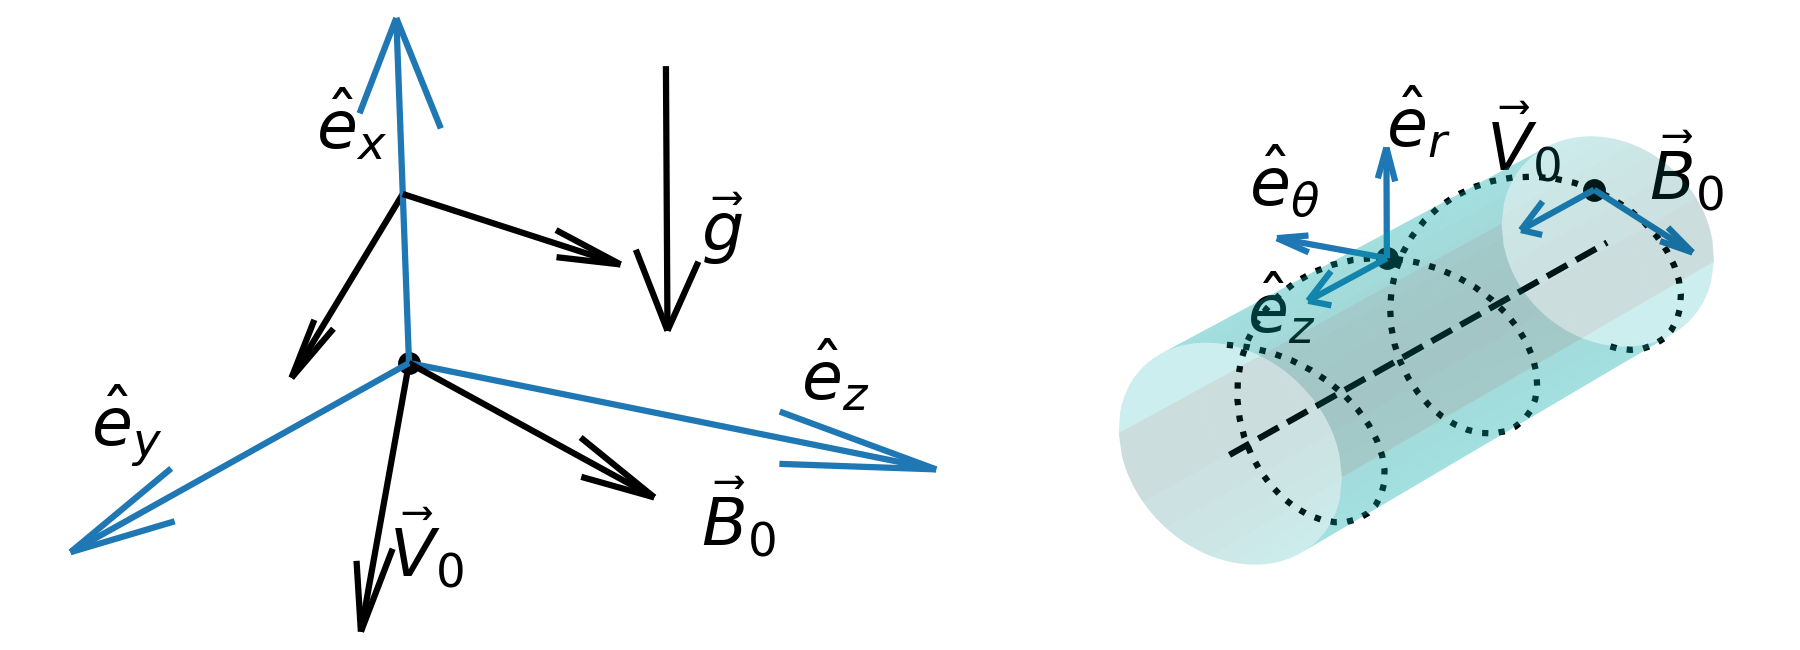
\includegraphics[width=\textwidth]{coordinate_axes.png}
  \caption{
    Unit vectors and examples of $\bb_0$ and $\bv_0$ for the Cartesian (\textbf{left}) and cylindrical (\textbf{right}) cases. These correspond to the general formalism given by Equation \eqref{eq: legolas_equilibrium}
    with $v_{01} = B_{01} = 0$.
  }
  \label{fig: coordinate_axes}
\end{figure}

In what follows the $v_{01}(u_1)$ and $B_{01}$ terms are included in the mathematical formalism for completeness, but will be set to zero in all applications discussed in the remainder of this thesis. Essentially, this implies that the general formalism in Equation \eqref{eq: legolas_equilibrium} reduces to the configuration shown on Figure \ref{fig: coordinate_axes}.

\subsubsection{Resistive terms}
The resistivity contribution in the energy equation is given by $\gmone \eta (\nabla \times \bb)^2$, which can be straightforwardly linearised as
\begin{equation}
  \begin{gathered}
    \gmone\left(\eta_0 + \eta_1\right)\left(\nabla \times \bb_0 + \nabla \times \bb_1\right)^2 \\
    = 2\gmone \eta_0 \left(\nabla \times \bb_0\right) \cdot \left(\nabla \times \bb_1\right)
      + \gmone\eta_1 \left(\nabla \times \bb_0\right) \cdot \left(\nabla \times \bb_0\right),
  \end{gathered}
\end{equation}
in which the nonlinear terms and equilibrium contributions were omitted. For the resistivity $\eta$ one can in principle take any profile, {\legolas} implements the Spitzer resistivity given by
\begin{equation} \label{eq: spitzer_eta}
  \eta = \frac{4\sqrt{2\pi}}{3}\frac{
    Z_\text{ion} \electroncharge^2 \sqrt{\masse} \ln(\lambda)
  }{
    \left(4\pi\epsilon_0\right)^2\left(\boltzmanncte T\right)^{3/2}
  },
\end{equation}
where $Z_\text{ion}$ denotes the ionisation taken to be unity, $\electroncharge$ and $\masse$ denote the electron charge and mass, respectively, and $\epsilon_0$ and $\boltzmanncte$ are the electrical permittivity and Boltzmann constant. The Coulomb logarithm is given by $\ln(\lambda)$ and is approximately equal to 22 for solar coronal conditions \citep{book_MHD}. It is important to emphasise that, since we will further linearise the governing nonlinear equations, we can adopt fully realistic values for all the nonideal coefficients, such as the resistivity or thermal conduction coefficients. This is in contrast to fully nonlinear computations, which are severely restrained in reaching magnetic Reynolds numbers $\magneticreynolds$ beyond $10^4$--$10^5$. The assumption of Spitzer resistivity implies that the perturbed part $\eta_1$ can be written in terms of perturbed temperature as
\begin{equation}
  \eta_1 = \left.\frac{d\eta}{dT}\right|_{T_0}T_1.
\end{equation}

In addition to this {\legolas} allows for an anomalous resistivity prescription in which we typically have $\eta(\uunit{1}, \boldsymbol{j}(\uunit{1}, t))$, that is, a resistivity profile that is spatio-temporal in general, but for a fixed time, depends on position and current profile. This in turn implies that a total derivative should be used for the resistivity, given by
\begin{equation}
  \eta' = \frac{\partial \eta}{\partial u_1} + T_0'\frac{\partial \eta}{\partial T},
\end{equation}
when calculating the derivative with respect to $u_1$. In most use cases a resistivity profile $\eta(T(\uunit{1}))$ is sufficient however, which is only temperature dependent -- and hence indirectly spatially varying as well for inhomogeneous temperature profiles.

\subsubsection{Optically thin radiative losses}
Just as before the optically thin radiative losses are governed by the heat-loss function $\HLF$, and the radiative cooling term $\gmone \rho \HLF$ in the energy equation can be linearised as
\begin{equation}
  \gmone \rho_1 \HLF_0 + \gmone \rho_0 \HLF_1.
\end{equation}
This time however we generalise the formalism to include a density and temperature-dependent heating function
$\HLFheat(\rho, T)$, that is,
\begin{equation}
  \HLF = \rho\HLFcool - \HLFheat(\rho, T).
\end{equation}
{\legolas} has multiple cooling curves implemented, most notably {\jccorona} and {\spexdm} as shown on Figure \ref{fig: coolingcurves}. In addition a piecewise power law as described by \citet{rosner1978} is also implemented, which is an explicit (piecewise) function over the entire temperature domain.

\subsubsection{Anisotropic thermal conduction}
The thermal conduction term $\nabla \cdot (\bkappa \cdot \nabla T)$ in the energy equation is quite straightforward to linearise:
\begin{equation}
  \nabla \cdot \left(\bkappa_0 \cdot \nabla T_1\right) + \nabla \cdot \left(\bkappa_1 \cdot \nabla T_0\right).
\end{equation}
However, as we are dealing with a tensor quantity to model the anisotropy in MHD, the linearisation process is tricky. Rewriting the tensor expression \eqref{eq: conduction} as
\begin{equation}
  \bkappa = \left(\kappapara - \kappaperp\right)\unit{B}\unit{B} + \kappaperp\idmat,
\end{equation}
where $\unit{B} = \bb/B_0$ is the unit vector along the magnetic field. So in addition to having to linearise the thermal conduction coefficients, we \emph{also} have to linearise this unit vector to account for a change in tensor directions. This implies that $\unit{B}\unit{B}$ is linearised as
\begin{equation} \label{eq: linearised_eB}
  \begin{gathered}
    \underbrace{
      \unit{B$_0$}\unit{B$_0$}
      + \unit{B$_1$}\unit{B$_0$}
      + \unit{B$_0$}\unit{B$_1$}
    }_\text{``regular'' terms}
    \underbrace{
      - \unit{B$_0$}\unit{B$_0$}\left(\unit{B$_0$} \cdot \unit{B$_1$}\right)
      - \unit{B$_0$}\unit{B$_0$}\left(\unit{B$_1$} \cdot \unit{B$_0$}\right)
    }_\text{change in tensor directions} \\
    = \unit{B$_0$}\unit{B$_0$} + \unit{B$_1$}\unit{B$_0$} + \unit{B$_0$}\unit{B$_1$}
      - 2\unit{B$_0$}\unit{B$_0$}\left(\unit{B$_0$} \cdot \unit{B$_1$}\right).
  \end{gathered}
\end{equation}
In what follows we can use the identity
\begin{equation} \label{eq: divergence_expression}
  \nabla \cdot (\bb_0 f) = f\nabla \cdot \bb + \bb_0 \cdot \nabla f,
\end{equation}
with $f$ a scalar term, the first term drops out since $\nabla \cdot \bb = 0$. Additionally, to shorten the notation we introduce the symbol
\begin{equation}
  \kappapfK{j} \equiv \frac{\skappapara{j} - \skappaperp{j}}{B_0^2},
\end{equation}
in which $j$ is either 0 or 1, denoting the unperturbed or perturbed parts, respectively.

\paragraph{Unperturbed tensor part} This part is given by $\nabla \cdot \left(\bkappa_0 \cdot \nabla T_1\right)$, which becomes
\begin{equation}
  \begin{gathered}
    \nabla \cdot \Bigl[(\skappapara{0} - \skappaperp{0})\unit{B$_0$}\unit{B$_0$} \cdot \nabla T_1\Bigr]
      + \nabla \cdot (\skappaperp{0}\nabla T_1) \\
    = \bb_0 \cdot \nabla \left(\kappapfK{0} \bb_0 \cdot \nabla T_1\right)
      + \nabla \cdot \left(\skappaperp{0}\nabla T_1\right).
  \end{gathered}
\end{equation}


\paragraph{Perturbed tensor part} This is given by $\nabla \cdot \left(\bkappa_1 \cdot \nabla T_0\right)$ and can be worked out in a similar way as the unperturbed part. Substituting a vector potential $\bb_1 = \nabla \times \ba_1$ and combining Equation \eqref{eq: linearised_eB} with \eqref{eq: divergence_expression} yields
\begin{equation}
  \begin{gathered}
    \bb_0 \cdot \nabla \left(\kappapfK{1}\bb_0 \cdot \nabla T_0\right)
    + \nabla \cdot \left(\skappaperp{1} \nabla T_0\right) \\
    + \left(\nabla \times \ba_1\right) \cdot \nabla \left(\kappapfK{0} \bb_0 \cdot \nabla T_0\right)
    + \bb_0 \cdot \nabla \Bigl(\kappapfK{0}\left(\nabla \times \ba_1\right) \cdot \nabla T_0\Bigr) \\
    - \bb_0 \cdot \nabla \left[
      2\kappapfK{0}\frac{1}{B_0^2}\bb_0 \Bigl(\bb_0 \cdot (\nabla \times \ba_1)\Bigr) \cdot \nabla T_0
    \right].
  \end{gathered}
\end{equation}
Note that the first, third and last terms drop out if we have no $B_{01}$ component, since in that case
$\bb_0 \cdot \nabla T_0 = 0$, which in turn implies that there is no $\skappapara{1}$ contribution.
This is no longer the case if a constant $B_{01}$ component would be present, then all these terms are nonzero.

\paragraph{Perturbed conduction coefficients} If we assume Spitzer conductivity as in Equation \eqref{eq: thermal_coeffs}, i.e. $\kappapara(T)$ and $\kappaperp(\rho, T, \bb)$, then we can write the perturbed thermal conduction coefficients in terms of the other variables:
\begin{equation} \label{eq: short kappapara1}
  \skappapara{1} = \frac{\partial \kappapara}{\partial T} T_1,
\end{equation}
and
\begin{equation} \label{eq: short kappaperp1}
  \begin{aligned}
    \skappaperp{1} &=
      \frac{\partial \kappaperp}{\partial \rho}\rho_1
      + \frac{\kappaperp}{\partial T}T_1
      + \frac{\partial \kappaperp}{\partial B}\frac{\bb_0 \cdot \bb_1}{B} \\
    &= \frac{\partial \kappaperp}{\partial \rho}\rho_1
      + \frac{\kappaperp}{\partial T}T_1
      + 2\bb_0\cdot\bb_1 \frac{\partial \kappaperp}{\partial\left(B^2\right)},
  \end{aligned}
\end{equation}
where we used $\dfrac{\partial \kappaperp}{\partial (B^2)} = \dfrac{\partial \kappaperp}{\partial B}\dfrac{1}{2B}$.

\subsubsection{Additional physics}
It is worth noting that {\legolas} also includes a full Hall MHD treatment along with viscosity and viscous heating. We explicitly omit these additional physics in our current formalism, since adding the extra terms would lead to even longer equations; viscosity and Hall are also not used in any of the applications in this thesis. We give a (very) brief description of these additional terms here, but will not discuss them further.

The viscous force addition to the momentum equation is given in tensorial form by
$\mathbf{F}_{\mathrm{visc}} = -\nabla\cdot\left(\mu\mathbf{\Pi}\right)$, which for constant dynamic viscosity $\mu$ can be simplified to good approximation to
\begin{equation}
	\mathbf{F}_{\mathrm{visc}} \simeq \mu \left[ \nabla^2\bv + \frac{1}{3} \nabla\left(\nabla\cdot\bv\right)\right].
\end{equation}
This relies on splitting the tensor in a symmetric and antisymmetric part, as explained in \citet{porth2014_amrvac}. Linearising this yields
\begin{equation}
  \mu\left[\nabla^2\bv_1 + \frac{1}{3}\nabla(\nabla \cdot \bv_1)\right].
\end{equation}
In the energy equation we have a viscous heating term $\mu \left|\nabla \bv\right|^2$ on the right hand side, where we assume that the norm here (which is essentially the norm of a matrix) represents the Frobenius norm such that
\begin{equation}
  \mu\left|\nabla \bv\right|^2 = \mu\sum_{i=1}^{3}\sum_{j=1}^{3}\left(\nabla \bv\right)_{ij}^2,
\end{equation}
which can be linearised as
\begin{equation}
  2\mu\sum_{i=1}^{3}\sum_{j=1}^{3}\left(\nabla \bv_0\right)_{ij}\left(\nabla \bv_1\right)_{ij}
\end{equation}

The Hall contributions are added to the right-hand side of the induction equation, consisting of the regular Hall term, electron pressure term and electron inertia term
\begin{equation}
  -\frac{\eta_\text{H}}{\rho}(\nabla \times \bb) \times \bb
  + \frac{\eta_\text{H}}{\rho}\nabla p
  - \frac{\eta_\text{e}}{\rho}\frac{\partial (\nabla \times \bb)}{\partial t},
\end{equation}
respectively. The latter term introduces a temporal derivative and is brought to the left-hand side of the induction equation. The quantities $\eta_\text{H}$ and $\eta_\text{e}$ represent the Hall factor and electron inertia factor, respectively.




\subsection{Equilibrium conditions} \label{ss: equilibrium conditions}
To ensure the background is in magnetostatic equilibrium, we set the time-dependent parts of Equations \eqref{eq: continuity}--\eqref{eq: induction} to zero and fill in the expressions for the background. We do not consider resistive terms in the equilibrium prescription, which can be justified by considering that the time scale of these effects is considerably longer than the dynamical time scale of the system itself. The time scales on which the magnetic fields decay due to resistivity is much, much larger than the time scales of the resistive modes themselves. This is essentially a consequence of large magnetic Reynolds numbers $\magneticreynolds$ in typical astrophysical cases, yielding magnetic decay time scales of $\tau \sim \magneticreynolds \tau_\text{A}$ (with $\tau_\text{A}$ the typical Alfv\'en time in ideal MHD) compared to much faster resistive mode time scales of $\tau \sim \magneticreynolds^\alpha$ (where typically $0 < \alpha < 1$). We can hence consider the equilibrium itself to be independent of resistivity, which removes some stringent extra conditions on the energy and induction equations. From Equation \eqref{eq: legolas_equilibrium} it then follows that the equilibrium background conditions are given by
\begin{gather}
  \left(\eps v_{01}\right)'\rho_0 + \eps v_{01}\rho_0' = 0 \\
  \left(\rho_0 T_0 + \frac{1}{2}B_{02}^2 + \frac{1}{2}B_{03}^2\right)'
    + \rho_0\left(g + v_{01}v_{01}'\right)
    + \frac{\eps'}{\eps}\left(B_{02}^2
    - \rho_0 v_{02}^2\right) = 0 \\
  \frac{B_{01}}{\eps}\left(\eps B_{02}\right)' - \rho_0 v_{01}\left(\frac{\eps'}{\eps}v_{02} + v_{02}'\right) = 0 \\
  B_{01}B_{03}' - \rho_0 v_{01}v_{03}' = 0 \\
  T_0 \rho_0 \frac{\left(\eps v_{01}\right)'}{\eps}
    + \rho_0 \HLF_0
    - B_{01}^2\left(\kappapfK{0} T_0'\right)'
    - \frac{1}{\eps}\left(\eps \kappa_{\perp, 0} T_0'\right)'
    + \frac{1}{\gmone}T_0'\rho_0 v_{01} = 0, \label{eq: general_thermal_equilibrium} \\
  \left(B_{02}v_{01} - B_{01}v_{02}\right)' = 0, \\
  \Bigl[\eps \left(B_{01}v_{03} - B_{03}v_{01}\right)\Bigr]' = 0,
\end{gather}
where the prime denotes the derivative with respect to $u_1$. The above set of equations describe an equilibrium state for a generalised background. If we set $v_{01} = B_{01} = 0$ however, this reduces to only two conditions for the time-independent parts, given by
\begin{gather}
  \left(\rho_0 T_0 + \frac{1}{2}B_{02}^2 + \frac{1}{2}B_{03}^2\right)'
    + \rho_0 g
    + \frac{\eps'}{\eps}\left(B_{02}^2 - \rho_0 v_{02}^2\right) = 0, \label{eq: force_equilibrium} \\
  \rho_0 \HLF_0 - \frac{1}{\eps}\left(\eps \skappaperp{0} T_0'\right)' = 0. \label{eq: thermal_equilibrium}
\end{gather}
The first equation originates from the momentum equation \eqref{eq: momentum} and should always be satisfied as it expresses a force-balanced state. The second condition originates from the non-adiabatic terms in the energy equation and should (only) be accounted for if these terms are included. Note that the third term in Equation \eqref{eq: force_equilibrium} is only included for a cylinder, since $\eps' = 0$ in a Cartesian geometry. This translates to the well-known fact that the centrifugal and tensional parts of the Lorentz force are absent for a Cartesian slab. Furthermore a cylindrical equilibrium profile should satisfy on-axis regularity conditions, meaning that $v_{02}$, $v_{03}'$, $B_{02}$ and $B_{03}'$ all have to be equal to zero at $r = 0$. When considering an accretion disk in the cylindrical limit, the inner edge of the disk is at $r = 1$, so lengths are then expressed in this inner disk radius and no regularity conditions apply in that case.

\subsubsection{Implications on the radiative cooling terms}
It is worth discussing that we explicitly kept $\HLF_0$ in the equilibrium expressions. This term is actually needed to ensure a thermally stable state, and is \emph{not necessarily zero} but depends on the physical effects under consideration, in particular perpendicular thermal conduction and the choice of heating function. Generally speaking, the heating function $\HLFheat$ can be anything -- for example heating through dissipative Alfv\'en waves \citep{vanderholst2014} -- but since there is still no well-defined parametrisation for coronal heating to date this term can be assumed to be as convenient as possible, that is, constant in time but possibly varying in space to ensure thermodynamic balance. Note that $\HLFheat$ should always be consistent with a given equilibrium profile as to exactly balance out the radiative losses (and possibly the thermal conduction effects and/or ohmic heating terms), in order to reach a thermal equilibrium state. This indirectly implies that a constant heating term is not necessarily independent of location, but dependent on the connection between the radiative losses and equilibrium temperature profile, which, in general, are both spatially dependent. It is worth noting that the inclusion of time-dependent background heating (or flows for that matter) can influence the spectrum in itself, as shown in for example \citet{barbulescu2019, hillier2019}, but due to the time-dependence of those effects the assumption of a stationary background state is no longer applicable.

Depending on the heating function and presence of thermal conduction, we can distinguish between two main cases: a constant heating function or a heating function that varies with temperature and density.

\paragraph{Heating is constant}
Here we consider a constant heating term $\HLFheat$, such that
\begin{equation}
  \HLF_0 = \rho_0\Lambda(T_0) - \HLFheat_0
  \qquad
  \text{and}
  \qquad
  \frac{\partial \HLFheat}{\partial T} = \frac{\partial \HLFheat}{\partial \rho} = 0,
\end{equation}
so here we consider a (spatially varying) heating term, simply assumed to be locally constant such that the radiative cooling contribution is balanced out. This implies

\begin{enumerate}
  \item[\textbf{a)}] If $B_{01} = v_{01} = \skappaperp{0} = 0$, then we have $\HLFheat_0 = \rho_0\Lambda(T_0)$ such that $\HLF_0 = 0$. This is consistent with the requirement given in Equation \eqref{eq: thermal_equilibrium}.
  \item[\textbf{b)}] If any of $\{B_{01}, v_{01}, \skappaperp{0}\}$ is non-zero then $\HLFheat_0$ will have additional terms from Equation \eqref{eq: general_thermal_equilibrium} besides $\rho_0\Lambda(T_0)$, which implies that $\HLF_0 \neq 0$ and thus has to be taken into account.
\end{enumerate}

\paragraph{Heating is not constant}
Here we consider the general case where $\HLFheat(\rho, T)$ depends on density and temperature, that is,
\begin{equation}
  \HLF_0 = \rho_0\Lambda(T_0) - \left. \HLFheat(\rho, T)\right|_{\rho_0, T_0} + \mathcal{C}_\HLFheat
  \qquad
  \text{and}
  \qquad
  \frac{\partial \HLFheat}{\partial T} \neq 0,
  \quad
  \frac{\partial \HLFheat}{\partial \rho} \neq 0.
\end{equation}
For a general heating function $\HLFheat(\rho, T)$ the thermal balance equation \eqref{eq: general_thermal_equilibrium} is not necessarily satisfied when $\HLFheat$ is evaluated in the equilibrium profiles; hence we added the constant $\mathcal{C}_\HLFheat$ with as sole purpose to provide additional terms to make sure everything is balanced, and we can write this constant as
\begin{equation}
  \mathcal{C}_\HLFheat = \left.\HLFheat(\rho, T)\right|_{\rho_0, T_0} - \HLFheat_0.
\end{equation}
This can be thought of as splitting the heating term in a $(\rho ,T)$ dependent and independent part, and since $\mathcal{C}_\HLFheat$ is locally constant (but again, possibly spatially varying) it does not influence the temperature and density derivatives of $\HLFheat$. We can again distinguish between

\begin{enumerate}
  \item[\textbf{a)}] $B_{01} = v_{01} = \skappaperp{0} = 0$. From the thermal balance equation it follows that $\HLF = 0$ must hold. This therefore implies that $\HLFheat_0 = \rho_0 \Lambda(T_0)$ following Equation \ref{eq: thermal_equilibrium}.
  \item[\textbf{b)}] Any of $\{B_{01}, v_{01}, \skappaperp{0}\} \neq 0$. Similar to the constant heating case $\HLF_0 \neq 0$, and $\HLFheat$ has additional terms governed by Equation \eqref{eq: general_thermal_equilibrium}.
\end{enumerate}

For both constant and non-constant heating it holds that
\begin{equation} \label{eq: perturbed_HLF}
  \begin{aligned}
    \HLF_1 &= \left(
      \Lambda(T_0) - \left.\frac{\partial \HLFheat(\rho, T)}{\partial \rho}\right|_{\rho_0, T_0}
    \right)\rho_1 + \left(
      \rho_0 \left.\frac{\partial \HLFcool}{\partial T}\right|_{T_0}
      - \left.\frac{\partial \HLFheat(\rho, T)}{\partial T}\right|_{\rho_0, T_0}
    \right) T_1, \\
          &= \dHLFrho \rho_1 + \dHLFT T_1,
  \end{aligned}
\end{equation}
which for constant heating reduces to the previous expression \eqref{eq: dHLF_homogeneous}. For the remainder of this thesis we will only consider a constant term here: as convenient as possible so that thermal balance is satisfied, but possibly locally varying over the domain.

\subsection{The linearised equations}
With all the necessary terms calculated in the previous Section we are now in a position to linearise Equations \eqref{eq: continuity}--\eqref{eq: induction} around the background specified by Equation \eqref{eq: legolas_equilibrium}. We again denote the unperturbed time-independent parts with a subscript 0 and the perturbed time-dependent parts with a subscript 1. It follows from the adopted equilibrium configuration that $\nabla \cdot \bb_0 = 0$, such that the divergence-free condition on the magnetic field is fulfilled and that the equilibrium flow field is compressible if
$v_{01} \neq 0$ and incompressible if $v_{01} = 0$. It should be noted that also in the latter case the perturbed quantities can represent both compressible and incompressible eigenoscillations. Furthermore the no-monopole condition should also be taken into account for the perturbed magnetic field, we therefore adopt a vector potential to write $\bb_1 = \nabla \times \ba_1$ such that $\nabla \cdot \bb_0 = 0$ is automatically satisfied. The system of linearised equations is then given by

{\customEquationFont

\begin{equation} \label{eq: linearised_continuity}
  \frac{\partial \rho_1}{\partial t} = -\nabla \cdot (\rho_0 \bv) - \nabla \cdot (\rho_1 \bv),
\end{equation}

\begin{equation} \label{eq: linearised_momentum}
  \begin{aligned}
    \rho_0\frac{\bv_1}{\partial t} =&
      -\nabla(T_0\rho_1 + \rho_0 T_1)
      - \rho_0 \bv_0 \cdot \nabla\bv_1
      - \rho_0\bv_1 \cdot \nabla \bv_0
      - \rho_1 \bv_0 \cdot \nabla \bv_0 \\
      \quad&
      + \rho_1 \bg
      + (\nabla \times \bb_0) \times (\nabla \times \ba_1)
      + [\nabla \times (\nabla \times \ba_1)] \times \bb_0,
  \end{aligned}
\end{equation}

\begingroup
\allowdisplaybreaks
\begin{equation} \label{eq: linearised_energy}
  \begin{aligned}
    \rho_0\frac{\partial T_1}{\partial t} =&
      - \rho_0\bv_1 \cdot \nabla T_0
      - \rho_0 \bv_0 \cdot \nabla T_1
      - \gmone\rho_0 T_0 \nabla \cdot \bv_1 \\
      \quad&
      - \gmone(T_0 \rho_1 + \rho_0 T_1)\nabla \cdot \bv_0
      - \gmone\rho_1 \HLF_0 \\
      \quad&
      - (\gamma - 1)\rho_0(\dHLFrho \rho_1 + \dHLFT T_1)
      + \gmone \bb_0 \cdot \nabla\left(\kappapfK{0}\bb_0 \cdot \nabla T_1 \right) \\
      \quad&
      + \gmone \nabla \cdot \left(\skappaperp{0}\nabla T_1\right)
      + \gmone \bb_0 \cdot \nabla \left(\kappapfK{1} \bb_0 \cdot \nabla T_0\right) \\
      \quad&
      + \gmone \nabla \cdot \left(\skappaperp{1} \nabla T_0\right)
      + \gmone \left(\nabla \times \ba_1\right) \cdot \nabla \left(\kappapfK{0}\bb_0 \cdot \nabla T_0\right) \\
      \quad&
      + \gmone \bb_0 \cdot \nabla \left[\kappapfK{0}\left(\nabla \times \ba_1\right) \cdot \nabla T_0\right] \\
      \quad&
      - \gmone \bb_0 \cdot \nabla \left[
        2\kappapfK{0}\frac{1}{B_0^2}\bb_0\bigl(\bb_0 \cdot \left(\nabla \times \ba_1\right)\bigr) \cdot \nabla T_0
      \right] \\
      \quad&
      + 2 \gmone \eta_0 \left(\nabla \times \bb_0\right)\cdot \left[\nabla \times \left(\nabla \times \ba_1\right)\right]
      + \gmone \frac{d\eta}{dT}T_1\left(\nabla \times \bb_0\right)^2, \\
  \end{aligned}
\end{equation}
\endgroup

\begin{equation} \label{eq: linearised_induction}
  \frac{\partial \ba_1}{\partial t} =
    \bv_1 \times \bb_0
    + \bv_0 \times \left(\nabla \times \ba_1\right)
    - \eta_0 \nabla \times \left(\nabla \times \ba_1\right)
    - \frac{d\eta}{dT}T_1 \nabla \times \bb_0.
\end{equation}
}


\subsubsection{Selfgravity extension}
Note that the above set of linearised equations \eqref{eq: linearised_continuity}--\eqref{eq: linearised_induction} assumed an external gravitational field, so we did not need to linearise the gravity term $\bg$ -- this is the so-called \emph{Cowling approximation}. However, in some cases instabilities may be driven by the self-gravity of the system, an example of which is the well-known Jeans instability which dates back to seminal work done by \citet{book_jeans}. {\legolas} can actually investigate these sort of instabilities through a modification of the original set of MHD equations. This is done through a linearisation of the gravitational term $\bg$ to $\bg_0 + \bg_1$, which essentially adds an additional variable to the system. The system is closed again by adding the Poisson equation $\nabla \cdot \bg = -4\pi \gravG \rho$ as a ninth equation to the existing set, with $\gravG$ the gravitational constant. If now a gravitational potential $\Phi$ is introduced as $\bg = -\nabla \Phi$, this implies that the ninth equation added to the system is given by
\begin{equation}
  \nabla^2\Phi_1 = 4\pi\rho_1,
\end{equation}
in normalised units. In order to connect this new equation with the others we take the time derivative of both sides, which introduces a temporal derivative of $\rho_1$. The continuity equation is substituted in, such that the final linearised form of the Poisson equation is given by
\begin{equation}
  \frac{\partial \nabla^2 \Phi}{\partial t} =
    -4\pi \Bigl[\nabla \cdot \left(\rho_0 \bv_1\right) + \nabla \cdot \left(\rho_1 \bv_0\right)\Bigr],
\end{equation}
and an additional term $-\rho_0 \nabla \Phi_1$ is added on the right hand side of the momentum equation \eqref{eq: linearised_momentum}.

The above formalism is included for completeness, although we will not use selfgravity in any of the applications in this thesis. The gravitational potential and Poisson equation will be omitted from the equations that follow and we will stick to the Cowling approximation; however, the corresponding matrix elements will be given in the Appendices.

\section{Obtaining the eigenvalue problem} \label{sec: eigenvalue problem}
In this Section we will go in-depth on how the eigenvalue problem arises from the above set of linearised equations.
The main idea here is similar to what we did in Chapter \ref{ch: spectroscopy}: now that we have expressions for the linearised equations we can perform a Fourier analysis in the ignorable coordinates, which will give us an eigenvalue problem that can be solved to obtain all modes in the system under consideration. At first glance this may look quite straightforward to do; however, as will become clear in the sections that follow, every step in this process introduces numerical and mathematical challenges that have to be overcome first.

\subsection{Fourier analysis} \label{ss: fourier}
The first step in the eigenvalue approach is to perform a Fourier analysis with an exponential time dependence on the above set of linearised equations, imposing standard Fourier modes on the $u_2$ and $u_3$ coordinates of a perturbed quantity $f_1$, given by
\begin{equation} \label{eq: fourier_analysis}
  f_1 = \hat{f_1}(u_1)\exp\Bigl[\icomplex(k_2 u_2 + k_3 u_3 - \omega t)\Bigr].
\end{equation}
In this form the wave numbers $k_2$ and $k_3$ correspond to $k_y$ and $k_z$ in Cartesian geometry, and to $m$ and $k$ in a cylindrical geometry. Note that $m$ is quantified to integer values, since the $\theta$-direction is periodic. For reasons that will become clear in a moment, we apply the following transformation to the perturbed quantities
\begin{equation}
  \begin{alignedat}{4} \label{eq: transformation}
    \eps \rho_1 &= \widetilde{\rho_1},
    \qquad&
    \icomplex \eps v_1 &= \widetilde{v_1},
    \qquad&
    v_2 &= \widetilde{v_2},
    \qquad&
    \eps v_3 &= \widetilde{v_3}, \\
    \eps T_1 &= \widetilde{T_1},
    &
    \icomplex a_1 &= \widetilde{a_1},
    &
    \eps a_2 &= \widetilde{a_2},
    &
    a_3 &= \widetilde{a_3}. \\
  \end{alignedat}
\end{equation}
This particular transformation simplifies the resulting set of equations and has as additional effect that all adiabatic and incompressible flow terms are real, such that we are only dealing with imaginary terms if resistivity or non-adiabatic effects are included. This is in analogy to the fact that the purely adiabatic case is governed by self-adjoint operators: one for the case without flow and two for the case with flow included \citep{goedbloed2018_web1,goedbloed2018_web2}. For brevity we introduce the following quantities
\begin{equation} \label{eq: F_G_operators}
  \Fplus \equiv \Fplusfull,
  \qquad
  \Gmin \equiv \Gminfull,
\end{equation}
as is common notation in MHD spectral theory following \citet{book_MHD}. These symbols essentially represent the parallel ($\Fplus$) and perpendicular ($\Gmin$) parts of the gradient operator applied to a perturbed quantity, with terms originating from the exponential Fourier factor. In other words, we could write $B_0 \kpara = \Fplus$
and $B_0 \kperp = \Gmin$. We can introduce a similar symbol for the background flow field, given by
\begin{equation} \label{eq: V_operator}
  \Vplus \equiv \Vplusfull,
\end{equation}
which is similar to $\Fplus$ but now with flow terms instead of magnetic field terms.

The final set of Fourier-analysed linearised equations is given below, where the tilde notation in Equation \eqref{eq: transformation} is dropped for the sake of simplicity. From now on, tildes will no longer be written explicitly since there is no confusion possible.

\paragraph{Continuity equation}
{\customEquationFont
\begin{equation} \label{eq: full_continuity}
  \omega\rho_1 =
    -\rho_0' v_1 + \rho_0\left(k_2 v_2 + k_3 v_3 - v_1'\right)
    -\icomplex v_{01}\rho_1' + \rho_1 \left(\Vplus - \icomplex v_{01}'\right)
\end{equation}
}

\paragraph{Momentum-1 equation}
{\customEquationFont
\begin{equation} \label{eq: full_momentum1}
  \begin{aligned}
  \omega\rho_0 v_1 &=
    \eps\left(\frac{T_0 \rho_1}{\eps} + \frac{T_1 \rho_0}{\eps}\right)'
    + g \rho_1
    + \rho_0 \left(\Vplus - \icomplex v_{01}'\right)v_1 \\
    &\quad
		+ B_{02} \left\{
      - \frac{k_2 k_3}{\eps}a_2 + \frac{k_2^2}{\eps}a_3 + \Bigl[\eps\left(k_3a_1 - a_3'\right)\Bigr]'
    \right\}
    + \left(\eps B_{02}\right)'\left(k_3a_1 - a_3'\right)  \\
    &\quad
    + B_{03} \left\{
      -k_3^2 a_2 + k_2 k_3a_3 + \eps\left[\frac{1}{\eps}\left(a_2' - k_2 a_1 \right)\right]'
    \right\}
    + B_{03}' \left(a_2' - k_2a_1\right) \\
    &\quad
    + \left(v_{01} v_{01}' - \frac{\eps' v_{02}^2}{\eps}\right)\rho_1
		- 2 \eps' \rho_0 v_{02} v_2
    - \icomplex \eps\rho_0 v_{01} \left(\frac{v_1}{\eps}\right)'
  \end{aligned}
\end{equation}
}

\paragraph{Momentum-2 equation}
{\customEquationFont
\begin{equation} \label{eq: full_momentum2}
  \begin{aligned}
  \omega\rho_0 \eps v_2 &=
    \frac{1}{\eps} k_2 T_0 \rho_1
    + \frac{1}{\eps}k_2 \rho_0 T_1
    + \icomplex B_{01} \left\{
      -\frac{k_2 k_3}{\eps}a_2  + \frac{k_2^2}{\eps}a_3 + \Bigl[\eps\left(k_3 a_1  - a_3'\right)\Bigr]'
    \right\} \\
    &\quad
    + B_{03} \left[- \left(\frac{k_2^2}{\eps} + \eps k_3^2\right)a_1  + \frac{ k_2}{\eps}a_2' +  \eps k_3a_3'\right]
    + \frac{(\eps B_{02})'}{\eps}\left(a_2 k_3 - a_3 k_2\right) \\
    &\quad
    - \frac{\left(\eps v_{02}\right)'}{\eps} \left(\icomplex v_{01} \rho_1 + \rho_0 v_1\right)
    + \eps\rho_0 \left(\Vplus - \icomplex \frac{\eps'}{\eps} v_{01}\right)v_2
    - \icomplex \eps \rho_0 v_{01} v_2'
  \end{aligned}
\end{equation}
}


\paragraph{Momentum-3 equation}
{\customEquationFont
\begin{equation} \label{eq: full_momentum3}
  \begin{aligned}
    \omega \rho_0 v_3 &=
      k_3 T_0 \rho_1
      + k_3 \rho_0 T_1
		  + B_{03}' \left(k_3 a_2  - k_2 a_3\right)
      - \icomplex v_{01} v_{03}' \rho_1
      - \rho_0 v_{03}'v_1 \\
      &\quad
		  + B_{02} \left[
        \left(\frac{k_2^2}{\eps} + \eps k_3^2\right)a_1  - \frac{k_2}{\eps}a_2'  - \eps k_3 a_3'
      \right]
      + \rho_0 v_3 \Vplus \\
		&\quad
    + \icomplex B_{01} \left[
      -k_3^2 a_2  + k_2 k_3 a_3  + \eps\left(- \frac{k_2}{\eps}a_1 + \frac{a_2'}{\eps}\right)'
    \right]
    - \icomplex \eps \rho_0 v_{01} \left(\frac{v_3}{\eps}\right)'
  \end{aligned}
\end{equation}
}

{\customEquationFont
\paragraph{Energy equation}
\begin{equation} \label{eq: full_energy}
  \begin{aligned}
    \omega\rho_0T_1 &=
    \gmone T_0 \rho_0 \left(k_2 v_2 + k_3 v_3 -  v_1'\right) - T_0'\rho_0 v_1
    - \icomplex \eps \rho_0 v_{01} \left(\frac{T_1}{\eps}\right)' \\
    &
    - \frac{1}{\eps}\icomplex \gmone T_0 \left(\eps v_{01}\right)'\rho_1
    + \rho_0 \left(\Vplus - \icomplex \gmone\frac{\left(\eps v_{01}\right)'}{\eps} \right) T_1 \\
    &
    - \icomplex \gmone \dHLFT \rho_0 T_1  - \icomplex \gmone \left(\HLF_0 + \dHLFrho \rho_0\right) \rho_1 \\
    &
    + 2 \icomplex \gmone \eta_0 \Biggl\{ \Biggr.
      B_{03}'\left[-k_3^2a_2 + k_2 k_3 a_3 + \eps\left(-\frac{k_2}{\eps}a_1  + \frac{1}{\eps}a_2'\right)'\right] \\
    &
    + \frac{\left(B_{02} \eps\right)'}{\eps}\left[
      - \frac{k_2 k_3}{\eps}a_2 + \frac{k_2^2}{\eps} a_3 + \Bigl(\eps k_3 a_1 - \eps a_3'\Bigr)'
    \right] \Biggl. \Biggr\} \\
    &
    + \icomplex \gmone \left\{
      \left[B_{03}'^2 + \left(\frac{\left(B_{02} \eps\right)'}{\eps}\right)^2\right]\frac{d\eta}{dT} T_1
    + \eps B_{01}^2\left(\frac{2}{\eps}\kappapfK{0}T_1' - \frac{T_0'}{\eps B_0^2}\dkappaperpdrho \rho_1\right)'
    \right\} \\
    &
    + \icomplex \gmone \eps B_{01}\left\{
      \left[
        2 \icomplex \kappapfK{0}\left(\frac{\eps'}{\eps}\icomplex B_{01} + \Fplus\right)
        + \frac{B_{01}}{B_0^2}T_0'\left(\dkappaparadT - \dkappaperpdT\right)
      \right]\frac{T_1}{\eps}
    \right\}' \\
    &
    + 2\icomplex \gmone \eps B_{01}^2\Biggl\{
      \frac{T_0'}{B_0^2}\left(\kappapfK{0} + \dkappaperpdB\right)
      \Biggl[\frac{\icomplex B_{01}}{\eps}\left(k_3 a_2 - k_2 a_3\right) + B_{02}a_3' \Biggr.\Biggr. \\
    &
      \Biggl. \Biggl. - \frac{B_{03}}{\eps}a_2' + \Gmin a_1\Biggr]\Biggr\}
    - \icomplex \gmone \left[
      \kappapfK{0}\Fplus^2
      + \skappaperp{0}\left(\frac{k_2^2}{\eps^2} + k_3^2\right)
    \right] T_1 \\
    &
    + \gmone \kappapfK{0} \eps B_{01} T_0' \left[
        -\frac{2 a_1}{B_0^2}\Fplus\Gmin - \frac{a_2'}{\eps}\left(k_3 - \frac{2 B_{03}}{B_0^2}\Fplus\right)
        + a_3'\left(\frac{k_2}{\eps} - \frac{2 B_{02}}{B_0^2}\Fplus\right)
    \right] \\
    &
    + \icomplex \gmone \kappapfK{0}T_0'\left(1 - 2\frac{B_{01}^2}{B_0^2}\right)\Fplus\left(k_3 a_2 - k_2 a_3\right)
    - \gmone \kappapfK{1}\eps B_{01}T_0'\Fplus \\
    &
    - \gmone \kappapfK{0} \eps B_{01} \Fplus \left(\frac{T_1}{\eps}\right)'
    + \gmone B_{01}\left(T_0' \kappapfK{0}\right)' \left(k_3 a_2 - k_2 a_3\right) \\
    &
    + \icomplex \gmone \left(T_0' \skappaperp{1}\eps\right)'
    + \icomplex \gmone \left[\skappaperp{0}\eps \left(\frac{T_1}{\eps}\right)'\right]',
  \end{aligned}
\end{equation}
}

\paragraph{Induction-1 equation}
{\customEquationFont
\begin{equation} \label{eq: full_induction1}
  \begin{aligned}
    \omega \eps a_1 &=
      B_{02}v_3 - \eps B_{03}v_2
      + \eps\Vplus a_1  - v_{02}a_2' - \eps v_{03}a_3'
      - \icomplex \eta_0 \left(\frac{k_2^2}{\eps} + \eps k_3^2\right)a_1 \\
      &\quad
      + \icomplex \eta_0 \frac{k_2}{\eps} a_2' + \icomplex \eta_0 \eps k_3 a_3'
  \end{aligned}
\end{equation}
}

\paragraph{Induction-2 equation}
{\customEquationFont
\begin{equation} \label{eq: full_induction2}
  \begin{aligned}
    \omega a_2 &=
    \icomplex B_{01} v_3 - B_{03} v_1
      + \icomplex k_2 v_{01}a_1 + k_3 v_{03} a_2 - \icomplex v_{01} a_2' - k_2 v_{03} a_3 \\
      &\quad
      + \icomplex B_{03}' \frac{d\eta}{dT} T_1
      - \icomplex \eta_0 k_3^2 a_2
      + \icomplex \eta_0 k_2 k_3 a_3
      + \icomplex \eta_0\eps \left(- \frac{k_2}{\eps}a_1  + \frac{1}{\eps}a_2'\right)'
  \end{aligned}
\end{equation}
}

\paragraph{Induction-3 equation}
{\customEquationFont
\begin{equation} \label{eq: full_induction3}
  \begin{aligned}
    \omega \eps a_3 &=
    - \icomplex \eps B_{01} v_2 + B_{02} v_1
    + \icomplex \eps k_3 v_{01} a_1
    - k_3 v_{02} a_2
    + k_2 v_{02} a_3
    - \icomplex v_{01} a_3' \\
    &\quad
    - \icomplex T_1 \frac{d\eta}{dT} \frac{\left(B_{02} \eps\right)'}{\eps}
    + \icomplex \eta_0 \frac{k_2 k_3}{\eps} a_2
    - \icomplex \eta_0 \frac{k_2^2}{\eps}a_3
    - \icomplex \eta_0 \Bigl(\eps k_3 a_1 - \eps a_3'\Bigr)'.
  \end{aligned}
\end{equation}
}

In the energy equation the terms $\skappapara{1}$ and $\skappaperp{1}$ are given by Equations \eqref{eq: short kappapara1} and \eqref{eq: short kappaperp1}, respectively. We now have a system of eight differential equations in $u_1$ for the perturbed quantities $\rho_1$, $v_1$, $v_2$, $v_3$, $T_1$, $a_1$, $a_2$ and $a_3$. If selfgravity is taken into account, the Fourier-analysed Poisson equation forms the ninth expression and adds the gravitational potential $\Phi_1$ as a ninth perturbed quantity.

At this point the actual scope of the problem should become clear, and a first major obstacle emerges: Equations \eqref{eq: full_continuity}--\eqref{eq: full_induction3} may look like an eigenvalue problem in $\omega$, with the quantities on the left-hand side of the equations composing the $\bmat$-matrix, those on the right-hand side of the equal sign the $\amat$-matrix, and the state vector given by $\statevec = (\rho_1, v_1, v_2, v_3, T_1, a_1, a_2, a_3)$. However, we actually have first and second order $u_1$-derivatives of the equilibrium quantities \emph{and} the state vector variables \emph{inside} the matrices.
Before we can solve for the eigenfrequencies $\omega$, we first have to rewrite the above set of equations in a proper generalised matrix eigenvalue problem; this is done using a finite element discretisation.


\subsection{Finite element analysis} \label{ss: finite_elements}
The system of Equations \eqref{eq: full_continuity}--\eqref{eq: full_induction3} actually defines a generalised complex eigenvalue problem in $\omega$ of the form $\amat \statevec = \omega \bmat \statevec$ in which the state vector $\statevec$ is given by
\begin{equation} \label{eq: statevector}
  \statevec = \left(\rho_1, v_1, v_2, v_3, T_1, a_1, a_2, a_3\right)
   = \left(x^1, x^2, x^3, x^4, x^5, x^6, x^7, x^8\right),
\end{equation}
where we used a specific notation such that the superscript on the right-hand side denotes the index of the unknown variable in the state vector (where we start counting from one). The matrices $\amat$ and $\bmat$ contain the various equilibrium quantities and differential operators with respect to $u_1$. The eigenvalue problem is rewritten using the finite element method (\gls{FEM}). The basic idea is to discretise the domain in (not necessarily equally spaced) subdomains that are separated by nodes, that is, prechosen fixed points $x_j$ with $j$ the node number ($0$ to $N$) on the interval $x$ (in the Cartesian case), after which a linear combination of basis functions is used to approximate the unknown variable $x^i$. These basis functions are represented by local piecewise polynomials on every subdomain and vanish outside this subdomain (hence the name ``finite'' elements). As shown in, for example, \citet{rappaz1977}, using the same basis functions for all variables leads to spectral pollution; this essentially implies that converged solutions $\omega_p$ are found which are not actually eigenvalues of the matrix. To avoid this one can use a combination of linear and constant finite elements, but as shown in \citet{kerner1985} this can yield inaccurate eigenvalues.
{\legolas} uses a combination of higher-order finite elements, namely quadratic basis functions for the variables $\rho_1, v_2, v_3, T_1, a_1$, and cubic Hermite basis functions for the variables $v_1, a_2, a_3$. The reasoning behind which variables are quadratic and which are cubic will become clear when we discuss the boundary conditions later on. The mixture of high-order finite elements ensures that the basis functions can represent certain physical properties of specific eigenfunctions exactly, and can, for example, allow for truly incompressible modes that have $\nabla \cdot \bv_1 = 0$ everywhere on the domain. The trade-off in using higher-order basis functions is that this not only increases the accuracy of the spectrum, but also increases the size of the final matrices by a factor of two compared to linear finite elements. One should therefore keep in mind that using even higher-order basis functions -- such as quartic or quintic splines -- may increase accuracy at lower resolutions, but the increased size of the matrices could mean that the solver may take an even longer time to reach a converged solution compared to lower-order basis functions at higher resolutions.

To summarise, the main idea behind a finite element approach is threefold:
\begin{enumerate}
  \item[i)] A specific domain is chosen, which is then discretised into subdomains of not necessarily equal spacing.
  \item[ii)] The (ordinary or partial) differential equations have their exact solutions approximated by a linear combination of basis functions, which consist of a certain choice of local piecewise polynomials that are zero outside of the subdomain under consideration.
  \item[iii)] When solving the system one obtains coefficients of the chosen linear combination, calculated such that the difference between the exact solution and the approximation ($\equiv$ \emph{the residual}) becomes minimal .
\end{enumerate}



\subsubsection{Variational analysis and Galerkin form}
Before proceeding with our analysis we hold a small mathematical interlude on variational analysis and look at how writing the problem in weak Galerkin form is quite convenient for our current formalism. An excellent journey through the basics of finite element methods can be found in \citet{book_fem1}, whereas \citet{book_MHD} give a thorough discussion on the Galerkin form; here we follow a similar reasoning and highlight the key ideas behind the weak formalism. Consider a given inhomogeneous differential equation of the form
\begin{equation} \label{eq: inhomo_diff_eq}
  -\bigl[p(u_1)x(u_1)'\bigr]' + q(u_1)x(u_1) - f(u_1) = 0,
\end{equation}
on an interval $u_1 \in [0, 1]$ for given (known) functions $p(u_1), q(u_1)$ and $f(u_1)$, where the prime denotes the derivative with respect to $u_1$. For simplicity think of the function $x(u_1)$ as one of the perturbed variables in one of the linearised equations, furthermore we assume the first and second order derivatives of $x(u_1)$ exist on
$[0, 1]$. If we were to solve the above equation on a domain discretised in $N$ subdomains, we would obtain an approximate solution $\hat{x}(u_1)$. In a finite element analysis this solution $\hat{x}(u_1)$ is given by a linear combination of basis functions. Before diving into the higher-order basis functions that {\legolas} uses, we first look at a simple linear basis function $h_i$ such that
\begin{equation} \label{eq: linear_basisfunctions}
  x(u_1) \approx \hat{x}(u_1) = \sum_{j = 0}^N x_j h_j(u_1),
\end{equation}
where $x_j$ are the coefficients in the linear combination. Note that $\hat{x}(u_1)$ is only an \emph{approximate solution}, so when we substitute this back into the original equation \eqref{eq: inhomo_diff_eq} this will not yield zero, but some $u_1$-dependent function instead. This is essentially the difference between the exact and approximate solution and is called the \emph{residual} $\hat{r}_s^N(u_1)$, given by
\begin{equation} \label{eq: residual}
  r_s^N(u_1) \equiv \sum_{j=0}^N x_j\left[-\Bigl(p(u_1)h_j'(u_1)\Bigr)' + q(u_1)h_j(u_1)\right] - f(u_1).
\end{equation}
The next question is quite straightforward: ``how can we calculate the coefficients $x_j$ in the linear combination, such that the residual becomes as close to zero as possible over our domain?'', which essentially implies that the approximate solution approaches the exact solution. This is usually done by requiring that the (sort of) averaged residual over the domain becomes zero, that is,
\begin{equation} \label{eq: weighted_residual_formalism}
  \int_0^1 w_k(u_1) r_s^N(u_1)du_1 = 0 \qquad\text{for}\qquad k = 0, 1 \ldots N,
\end{equation}
where $w_k$ is called a weight function, and the number of weight functions is taken to be equal to the number of coefficients $x_j$ in our approximate solution. This in turn implies that we now have $N + 1$ algebraic equations for $x_j$, which can be solved after selecting a weight function. The solution $\hat{x}(u_1)$ is said to converge if the residual vanishes in the limit $N \rightarrow \infty$ everywhere on the domain.

In principle one is free to choose any weight function; the special case where $w_k$ is taken equal to the basis function $h_k$ is called the \emph{Galerkin method}. The weighted residual formalism
\eqref{eq: weighted_residual_formalism} then takes on the expression
\begin{equation}
  -\sum_{j=0}^N\int_0^1 h_k x_j \frac{d}{du_1}\left(p\frac{dh_j}{du_1}\right)du_1
  + \sum_{j=0}^N\int_0^1 h_k x_j q h_j du_1
  - \sum_{j=0}^N\int_0^1 h_k f = 0,
\end{equation}
with the index $k$ ranging from 0 to $N$. The first term in this equation can be ``simplified'' further by performing integration by parts, which will also introduce a non-integral term that should be evaluated in the domain boundaries. These terms can in turn be exploited further, and we will come back to them when we discuss the boundary conditions. The formulation after applying integration by parts is called the \emph{weak Galerkin formalism}, and will be the main mathematical principle in our numerical approach. A convenient consequence of this formalism is that we are able to rewrite all second-order derivatives into combinations of integrals containing first-order derivatives and surface terms.

\subsection{The MHD equations in weak Galerkin form}
The above implies that if we rewrite our Fourier-analysed MHD equations using the Galerkin method they will change into a system of algebraic equations, which is eventually what we are aiming at. Noting that {\legolas} uses a combination of quadratic and cubic basis functions, we can approximate a state variable $x^i$ (with $i$ the state vector index) for a domain divided into $N$ subdomains (nodes) by
\begin{equation} \label{eq: linear_combo}
  x^i(u_1) \approx \sum_{j=0}^N \Bigl(H_j^1(u_1)x_{j1}^i + H_j^2(u_1)x_{j2}^i\Bigr),
\end{equation}
where $H_j^1(u_1)$ and $H_j^2(u_1)$ denote the quadratic or cubic elements at node $j$.
The cubic Hermite and quadratic basis functions themselves, hereafter denoted by $C_j$ and $Q_j$, respectively, are given by
\begingroup
\allowdisplaybreaks
\begin{align}
  Q^1_j(x) &=
  \begin{cases}
    \dfrac{4\left(x - x_{j-1}\right)\left(x_j - x\right)}{\left(x_j - x_{j-1}\right)^2}
    \qquad &\text{for}~ x_{j-1} \leq x \leq x_j,	\\
    0
    \qquad &\text{elsewhere},
  \end{cases} \label{eq: basisfunction_Q1} \\
  C^1_j(x) &=
  \begin{cases}
    \left(\dfrac{x - x_{j-1}}{x_j - x_{j-1}}\right)^2\left(3 - 2\dfrac{x - x_{j-1}}{x_j - x_{j-1}}\right)
    \qquad &\text{for}~ x_{j-1} \leq x \leq x_j,	\\
    \left(\dfrac{x_{j+1} - x}{x_{j+1} - x_j}\right)^2\left(3 - 2\dfrac{x_{j+1} - x}{x_{j+1} - x_j}\right)
    \qquad &\text{for}~ x_j \leq x \leq x_{j+1},	\\
    0
    \qquad &\text{elsewhere},
  \end{cases}	\label{eq: basisfunction_C1} \\
  Q^2_j(x) &=
  \begin{cases}
    \dfrac{\left(2x - x_j - x_{j-1}\right)\left(x - x_{j-1}\right)}{\left(x_j - x_{j-1}\right)^2}
    \qquad &\text{for}~ x_{j-1} \leq x \leq x_j,	\\
    \dfrac{\left(2x - x_{j+1} - x_j\right)\left(x - x_{j+1}\right)}{\left(x_{j+1} - x_j\right)^2}
    \qquad &\text{for}~ x_j \leq x \leq x_{j+1},	\\
    0
    \qquad &\text{elsewhere},
  \end{cases} \label{eq: basisfunction_Q2} \\
  C^2_j(x) &=
  \begin{cases}
    \left(x - x_j\right)\left(\dfrac{x - x_{j-1}}{x_j - x_{j-1}}\right)^2
    \qquad &\text{for}~ x_{j-1} \leq x \leq x_j,	\\
    \left(x - x_j\right)\left(\dfrac{x_{j+1} - x}{x_{j+1} - x_j}\right)^2
    \qquad &\text{for}~ x_j \leq x \leq x_{j+1},	\\
    0
    \qquad &\text{elsewhere},
  \end{cases} \label{eq: basisfunction_C2}
\end{align}
\endgroup
as in, for example, \citet{kerner1998} and \citet{book_MHD}, and are shown graphically along with their derivatives in Figure \ref{fig: basisfunctions}. Because we have two basis functions per subdomain, this allows for the approximation of both the original variable and its derivative by differentiation of Equation \eqref{eq: linear_combo}. Here it should also become clear why we are using the weak Galerkin formalism, as the integration by parts gets rid of any second-order derivatives.

\begin{figure}[t]
  \centering
  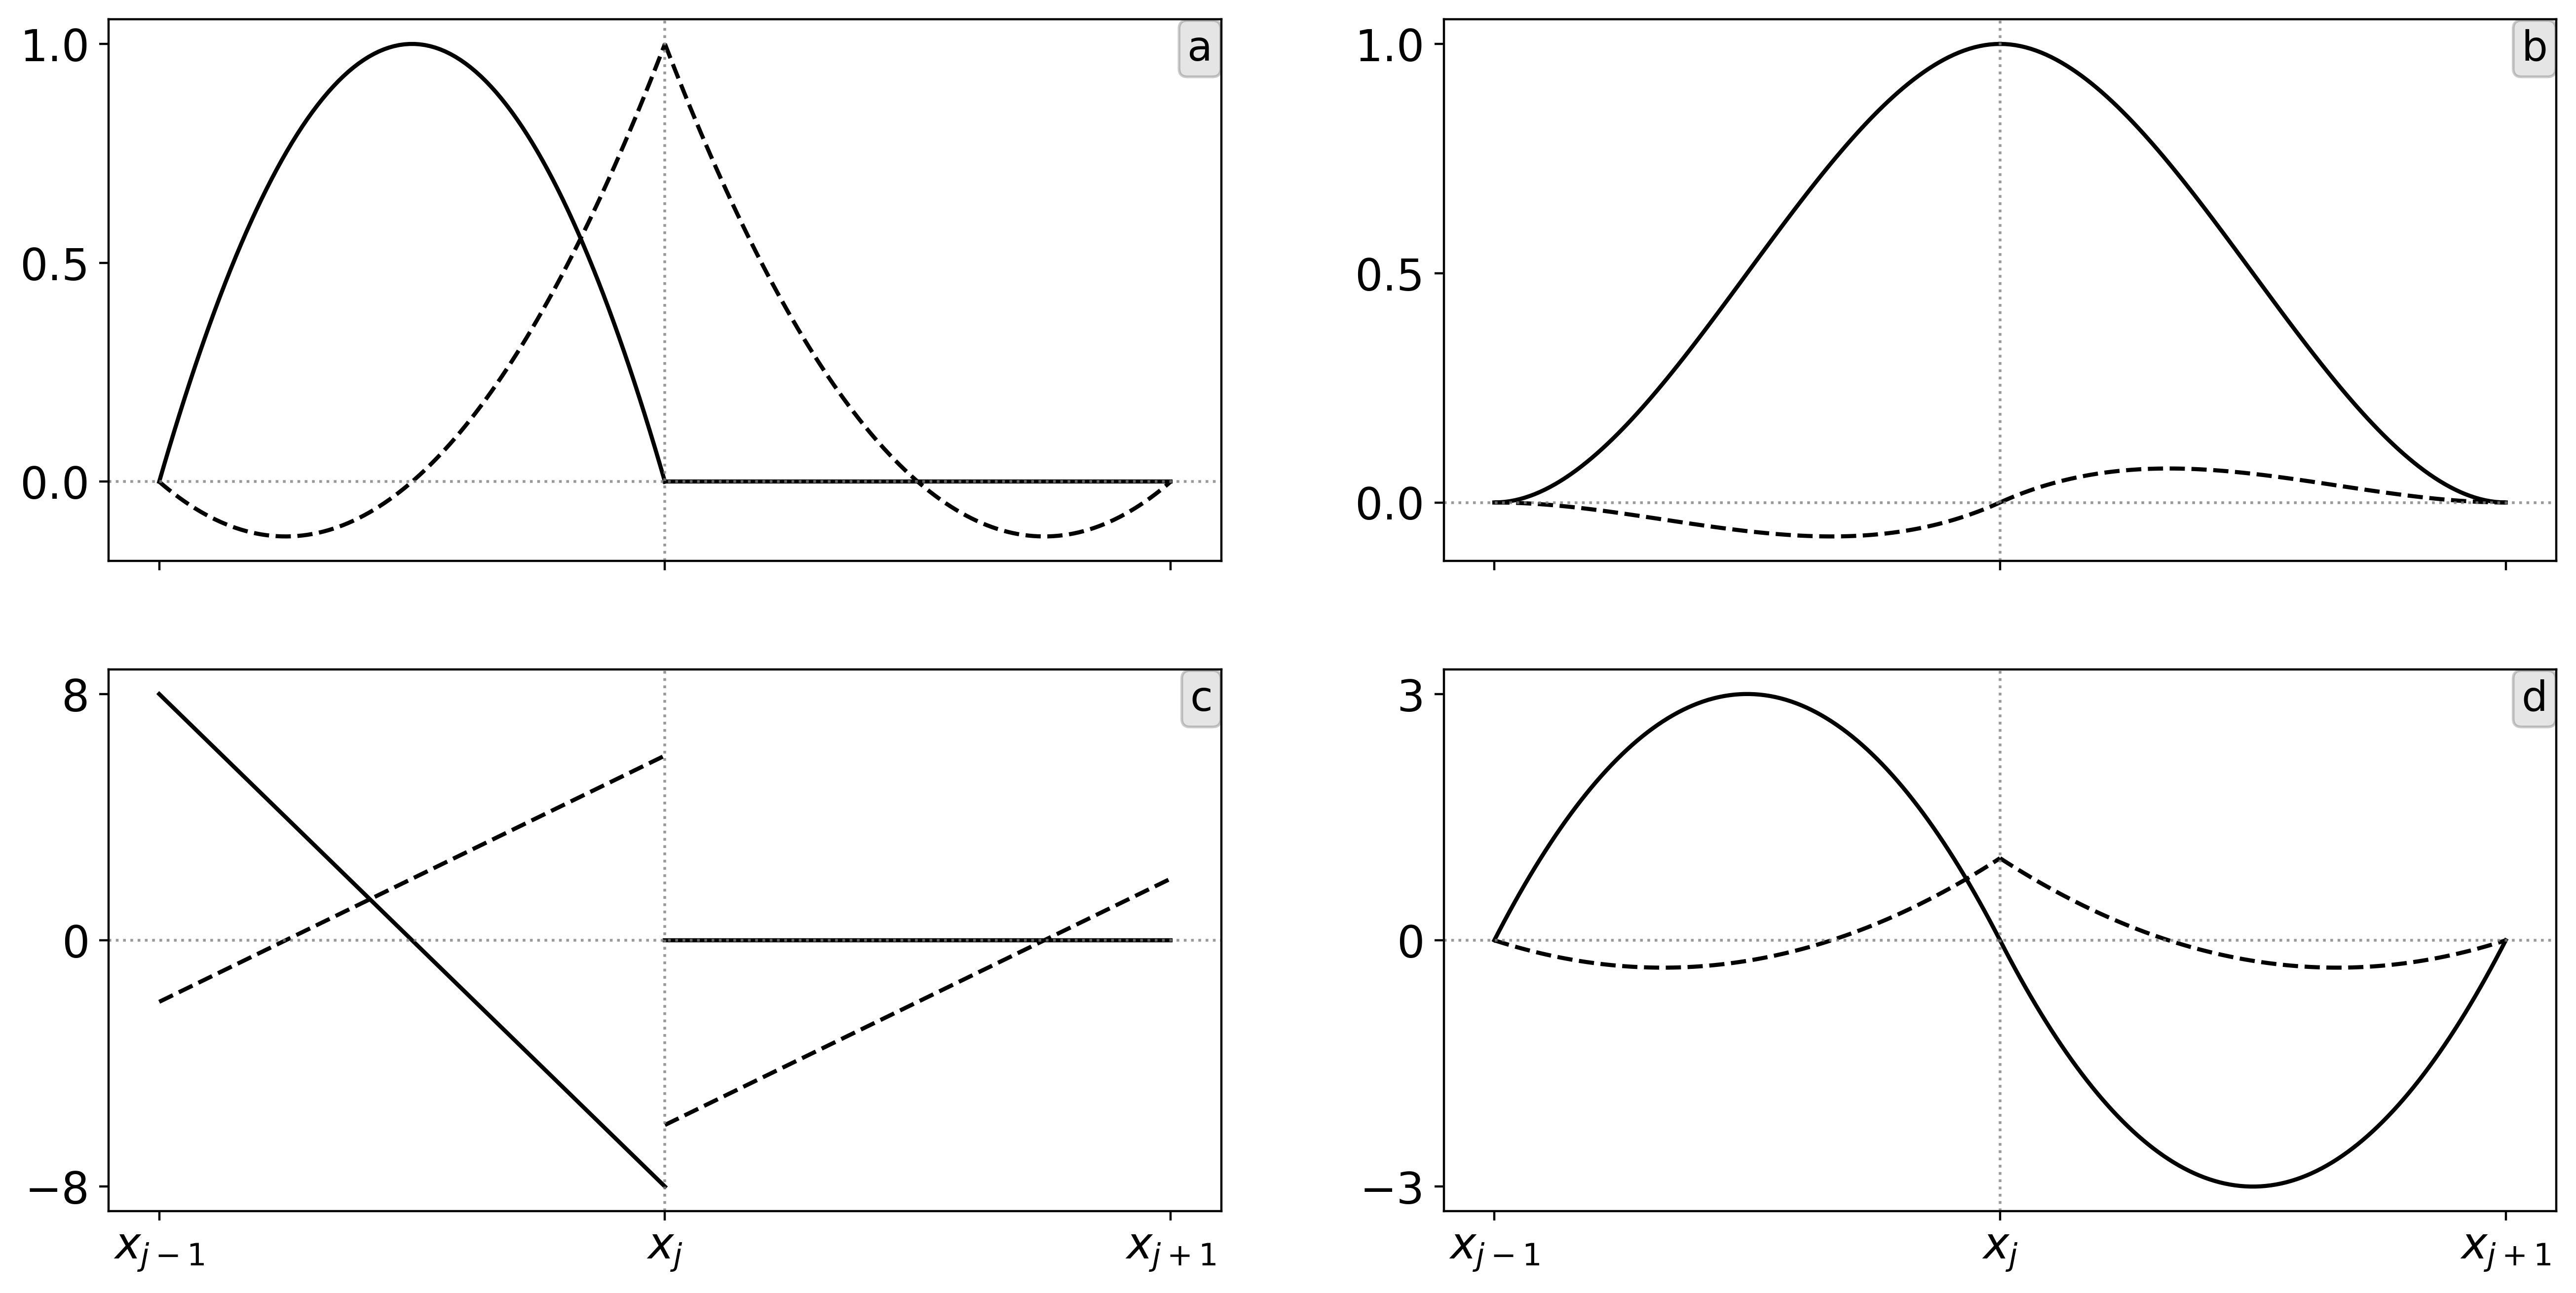
\includegraphics[width=\textwidth]{basisfunctions.png}
  \caption{
    The quadratic (\textbf{a}) and cubic (\textbf{b}) basis functions for the interval $[x_{j-1}, x_{j+1}]$ along with their derivatives (\textbf{c}) and (\textbf{d}), respectively. The solid lines denote $\{Q^1, C^1\}$, the dashed lines denote $\{Q^2, C^2\}$.
  }
  \label{fig: basisfunctions}
\end{figure}

We now proceed by rewriting our original set of equations \eqref{eq: full_continuity}--\eqref{eq: full_induction3} into weak Galerkin form. Each of the eight equations is multiplied by an appropriate element of the chosen basis (weight function), denoted by $h_j$, and integrate over the relevant domain. Because there are eight unknowns in our eigenvalue system, together with two basis functions and $N$ subdomains, this implies that the final matrix eigenvalue problem will have $16 N$ equations, resulting in a $16N \times 16N$ matrix. By extension, it becomes clear that using basis functions of even higher order will increase the size of this eigensystem considerably.

As an example we can write a part of the momentum-1 equation in weak Galerkin form. Because it is one of the simpler expressions and excellent as a short example, we consider the $T_1$ component on the right-hand side of Equation \eqref{eq: full_momentum1}, that is,
\begin{equation}
  \omega \rho_0 v_1 = \eps \left(\frac{\rho_0 T_1}{\eps}\right)'.
\end{equation}
These particular terms correspond to element $(2, 5)$ in the matrices. This ``number'' links to the indices of the state vector $\statevec$, because the momentum-1 equation is associated with $v_1$, or index $2$ in the state vector \eqref{eq: statevector}, and the $T_1$ component is associated with index $5$. As explained earlier we multiply the above equation with a weight function, and since we are using the Galerkin form this weight function is equal to the basis function, in this case the one associated with $v_1$ (i.e. a cubic polynomial), with notation $\hj{2}$. In the finite element representation adopted here, the $(v_1, T_1)$ contribution can be written as
\begin{equation} \label{eq: example_rho1_T1}
  \sum_{j=0}^N\omega \int \rho_0 \hj{2}\hk{2}du_1 =
  \sum_{j=0}^N\int \eps \hj{2}\left(\frac{\rho_0}{\eps}\hk{5}\right)'du_1,
\end{equation}
The $u_1$ dependence of the equilibrium density $\rho_0$ and basis functions $h^2$ and $h^5$ is implied. In this case, $h^2$ is cubic, because $v_1$ is associated with a cubic basis function; analogously $h^5$ is quadratic ($T_1$). The integrals are called \emph{matrix elements}, since the indices translate to the actual position in the final matrices of the eigenvalue problem. We will discuss this a little further in this section.

The matrix element corresponding to the left-hand side of Equation \eqref{eq: example_rho1_T1} can therefore be written as
\begin{equation}
  \bmat_{jk}(2, 2) = \int \rho_0 \hj{2}\hk{2}du_1,
\end{equation}
For the other side of the equal sign we can write the matrix element as
\begin{equation} \label{eq: amat_rho1_T1}
  \begin{aligned}
    \amat_{jk}(2, 5) &=
      \int \eps \hj{2}\left(\frac{\rho_0}{\eps}\hk{5}\right)'du_1, \\
      &\qquad \begin{cases}
        \text{u} = \eps\hj{2} \rightarrow \text{du} = \left(\eps'\hj{2} + \eps\dhj{2}\right)\text{d}u_1 \\
        \text{dv} = \left(\dfrac{\rho_0}{\eps}\hk{5}\right)'\text{d}u_1
          \rightarrow \text{v} = \dfrac{\rho_0}{\eps}\hk{5}
      \end{cases} \\
      &= \bigl.\rho_0 \hj{2}\hk{5}\bigr|_\Omega
        - \int \frac{\eps'}{\eps}\rho_0 \hj{2}\hk{5}du_1
        - \int \rho_0 \dhj{2}\hk{5}du_1,
  \end{aligned}
\end{equation}
where we applied integration by parts using the standard notation ``u'' and ``v'' to denote the parts, and the first term has to be evaluated over the domain $\Omega$.

The same strategy is applied to all equations in the linear system, from which it follows that $\bmat$ will only have equal-number matrix elements (i.e. only $(1, 1)$, $(2, 2)$, etc.), implying that $\bmat$ is fully symmetric and real. The $\amat$-matrix on the other hand, will have cross-term elements such that it is, in general, not symmetric. Furthermore, $\amat$ might be complex, depending on the included physical effects. Terms that contain derivatives of the state vector components, as for example $(v_1, T_1)$, are integrated by parts.

\subsubsection{Integrals through Gaussian quadrature}
When all the matrix elements have been calculated and the entire system is rewritten in the weak Galerkin form, then all elements of course contain one or more integrals that still have to be calculated. This is the next ``obstacle'' in our mathematical treatment: because the coefficient functions are in general quite complicated expressions depending on $u_1$ we have to suppose that the solutions of those integrals are not known, and can only be calculated analytically for very simple equilibrium expressions. A naive first idea could be to make use of Riemann sums, where we approximate a given integral by a finite sum of small regions, and for sufficiently small partitions (i.e. a large number of summation terms), this sum will asymptotically converge to the actual solution. However, we are dealing with \emph{a lot} of integrals, the number of which strongly scales with the finite element domain discretisation. While Riemann sums may sound like a good idea, they are quite cumbersome, slow, and will probably have a major performance impact on the assembly of the matrices.

A much better idea would be Gaussian quadrature, which essentially approximates the integral with a sum as well, but instead of area partitions it relies on Gaussian weights and nodes originating from the roots of the n-th degree Legendre polynomial; this allows for an \emph{exact} integration of degree $2n - 1$ polynomials \citep{book_MHD}. Additionally, it uses far fewer nodes compared to Riemann sums and is hence much more efficient both in terms of accuracy and calculations needed to achieve a solution due to a clever choice of weighting scheme. As Gaussian quadrature formalisms can be found in any standard textbook on numerical analysis, we will not go into much detail regarding the mathematical background and convergence properties. {\legolas} uses a four-point Gaussian quadrature to numerically approximate the integrals, and as such an integral in the interval $[x_{j-1}, x_j]$ can be expressed as
\begin{equation}
  \int_{x_{j-1}}^{x_j} f(u_1)du_1 \approx
    \frac{1}{2}\left(x_j - x_{j-1}\right)\sum_{i=1}^4 w_i f\left(
     \frac{1}{2}\left(x_j - x_{j-1}\right)\xi_i + \frac{1}{2}\left(x_{j-1} + x_j\right)
    \right),
\end{equation}
where $\xi_i$ and $w_i$ are the evaluation points (nodes) and weights of the 4-point Gaussian quadrature, given by
\begin{equation} \label{eq: gaussian_nodes}
  \begin{aligned}
    \left(\xi_i, w_i\right) &= \left(
      \pm \sqrt{\frac{3}{7} - \frac{2}{7}\sqrt{\frac{6}{5}}}, \frac{18 + \sqrt{30}}{36}
    \right)
    \approx (\pm 0.339981, 0.652145), \\
    \left(\xi_i, w_i\right) &= \left(
      \pm \sqrt{\frac{3}{7} + \frac{2}{7}\sqrt{\frac{6}{5}}}, \frac{18 - \sqrt{30}}{36}
    \right)
    \approx (\pm 0.861136, 0.347854).
  \end{aligned}
\end{equation}
The function $f$ denotes the integral coefficients, which are essentially the equilibrium quantities and basis functions evaluated in the various evaluation points.

\section{Assembly of the system}
Armed with the MHD equations in weak Galerkin form and detailed knowledge on the finite element treatment and how to approach the integrals, all that is left is putting the pieces together into a consistent formalism. The main goal here is to eventually obtain an eigenvalue problem in which both matrices purely consist of numbers, such that they can be passed on to various linear algebra solvers. At this point we have all matrix elements calculated, such that there are three steps remaining in the formalism:
\begin{itemize}
  \item[i)] \textbf{Matrix assembly}: Translate the matrix elements into actual positions within the matrices and evaluate the various integrals at the same time, thereby assembling the actual matrices $\amat$ and $\bmat$. Special attention must be given to how the finite element representation, matrix elements and locations in the matrices are interconnected.
  \item[ii)] \textbf{Boundary conditions}: We still have to specify proper boundary conditions and take care of the surface terms introduced through integration by parts.
  \item[iii)] \textbf{Eigenfunction assembly}: When the eigenvalue problem is solved, the eigenvectors are obtained within the finite element formalism and still have to be transformed to ``proper'' eigenfunctions.
\end{itemize}

\subsubsection{Matrix assembly}
The actual assembly of both matrices $\amat$ and $\bmat$ in {\legolas} is done by sequential iteration over the grid points. From Equations \eqref{eq: basisfunction_Q1}--\eqref{eq: basisfunction_C2}, we see that the finite elements have a localised nature around every grid point $j$, meaning that only the elements associated with a certain region (that is, the grid point $j$ itself and its neighbours $j - 1$ and $j + 1$) yield a nonzero contribution. However, it is actually easier implementation-wise to loop over the elements in the interval $[x_{j-1}, x_j]$ instead of over those in $[x_{j-1}, x_{j+1}]$, because then the actual integration of the matrix elements can be done in the same way, independent of whether the basis functions are cubic or quadratic. If only the interval $[x_{j-1}, x_j]$ is considered, we end up with 16 possible combinations of the basis functions for every grid point. This translates into a $4 \times 4$ submatrix for every variable, where every one of the 16 elements corresponds to one specific combination of the shape functions. As there are eight variables in the state vector, this implies a $32 \times 32$ matrix block for every grid point, hereafter dubbed a ``quadblock'' as it consists of four $16 \times 16$ blocks (hereafter called ``subblocks''). Every one of those subblocks inside a quadblock corresponds to a quarter section of the aforementioned submatrix, which is a $2 \times 2$ block in every subblock. Hence, to recap, a $2 \times 2$ block times eight variables represents a $16 \times 16$ subblock, of which four combined form a $32 \times 32$ quadblock for every grid point. Note that for the case of self-gravity we have nine equations, hence an $18 \times 18$ subblock and a $36 \times 36$ quadblock.

The Gaussian quadrature used to numerically approximate the integrals actually implies that every grid interval
$[x_{j-1}, x_j]$ is subdivided into four points, meaning that the equilibrium expressions are probed using $4(N - 1)$ points rather than $N$ points. The way the matrices are then assembled is thus done on a double-loop basis, where the outer loop iterates over the intervals $[x_{j-1}, x_j]$ and the inner loop iterates over the four Gaussian nodes. This inner loop calculates the basis functions and matrix elements at every point, then multiplies the coefficients with the Gaussian weights and finally adds them all together in a consistent manner. Because every quadblock corresponds to the interval $[x_{j-1}, x_j]$, we still have to account for the contribution of the $x_{j+1}$ grid point. This is done by partially overlapping the quadblock in the next grid point with the one from the previous grid point.

Figure \ref{fig: matrix_assembly} shows a visual representation of the structure and assembly process for the $\amat$-matrix, only six grid points were used for the purpose of illustration. Panel a shows the general matrix, highlighting the block-tridiagonal structure. The dashed grey lines denote the $32 \times 32$ quadblocks of the matrix, and every dot represents a nonzero value. In total, five quadblocks can be distinguished for six grid points, one for every grid interval. Panel b shows a zoom-in of the quadblock corresponding to the second grid interval as annotated on the left panel, where it can be seen that the top-left corner of this quadblock overlaps with the bottom-right corner of the previous quadblock corresponding to the first grid interval. A single quadblock is further divided into four subblocks, with the location of the different state variables annotated on Panel c of Figure \ref{fig: matrix_assembly}.
The matrix element $\amat(2, 5)$ is highlighted in every subblock, which corresponds to the $(v_1, T_1)$ contribution, which are cubic $(v_1)$ and quadratic $(T_1)$ variables. The $2 \times 2$ blocks in the top-left corner of the quadblock corresponds to the top-left $2 \times 2$ corner of the right panel, as indicated by the background colours. Panel c shows the various (16) combinations of the regular basis functions for a (cubic, quadratic) contribution, where the blue curve corresponds to the cubic basis functions and the orange curves to the quadratic ones. It should be noted that Panel c only shows one specific case, that is, the regular $\hj{2}\hk{5}$ terms of the matrix element. If, for example, the $\hj{2}\hk{7}$ element is calculated (which would be an $a_2$ term in the momentum-1 equation), the quadratic basis functions have to be replaced by their cubic counterparts, because $a_2$ is also a cubic variable. A similar reasoning can be made for the other matrix elements. \vfill

\begin{figure}[t!]
  \centering
  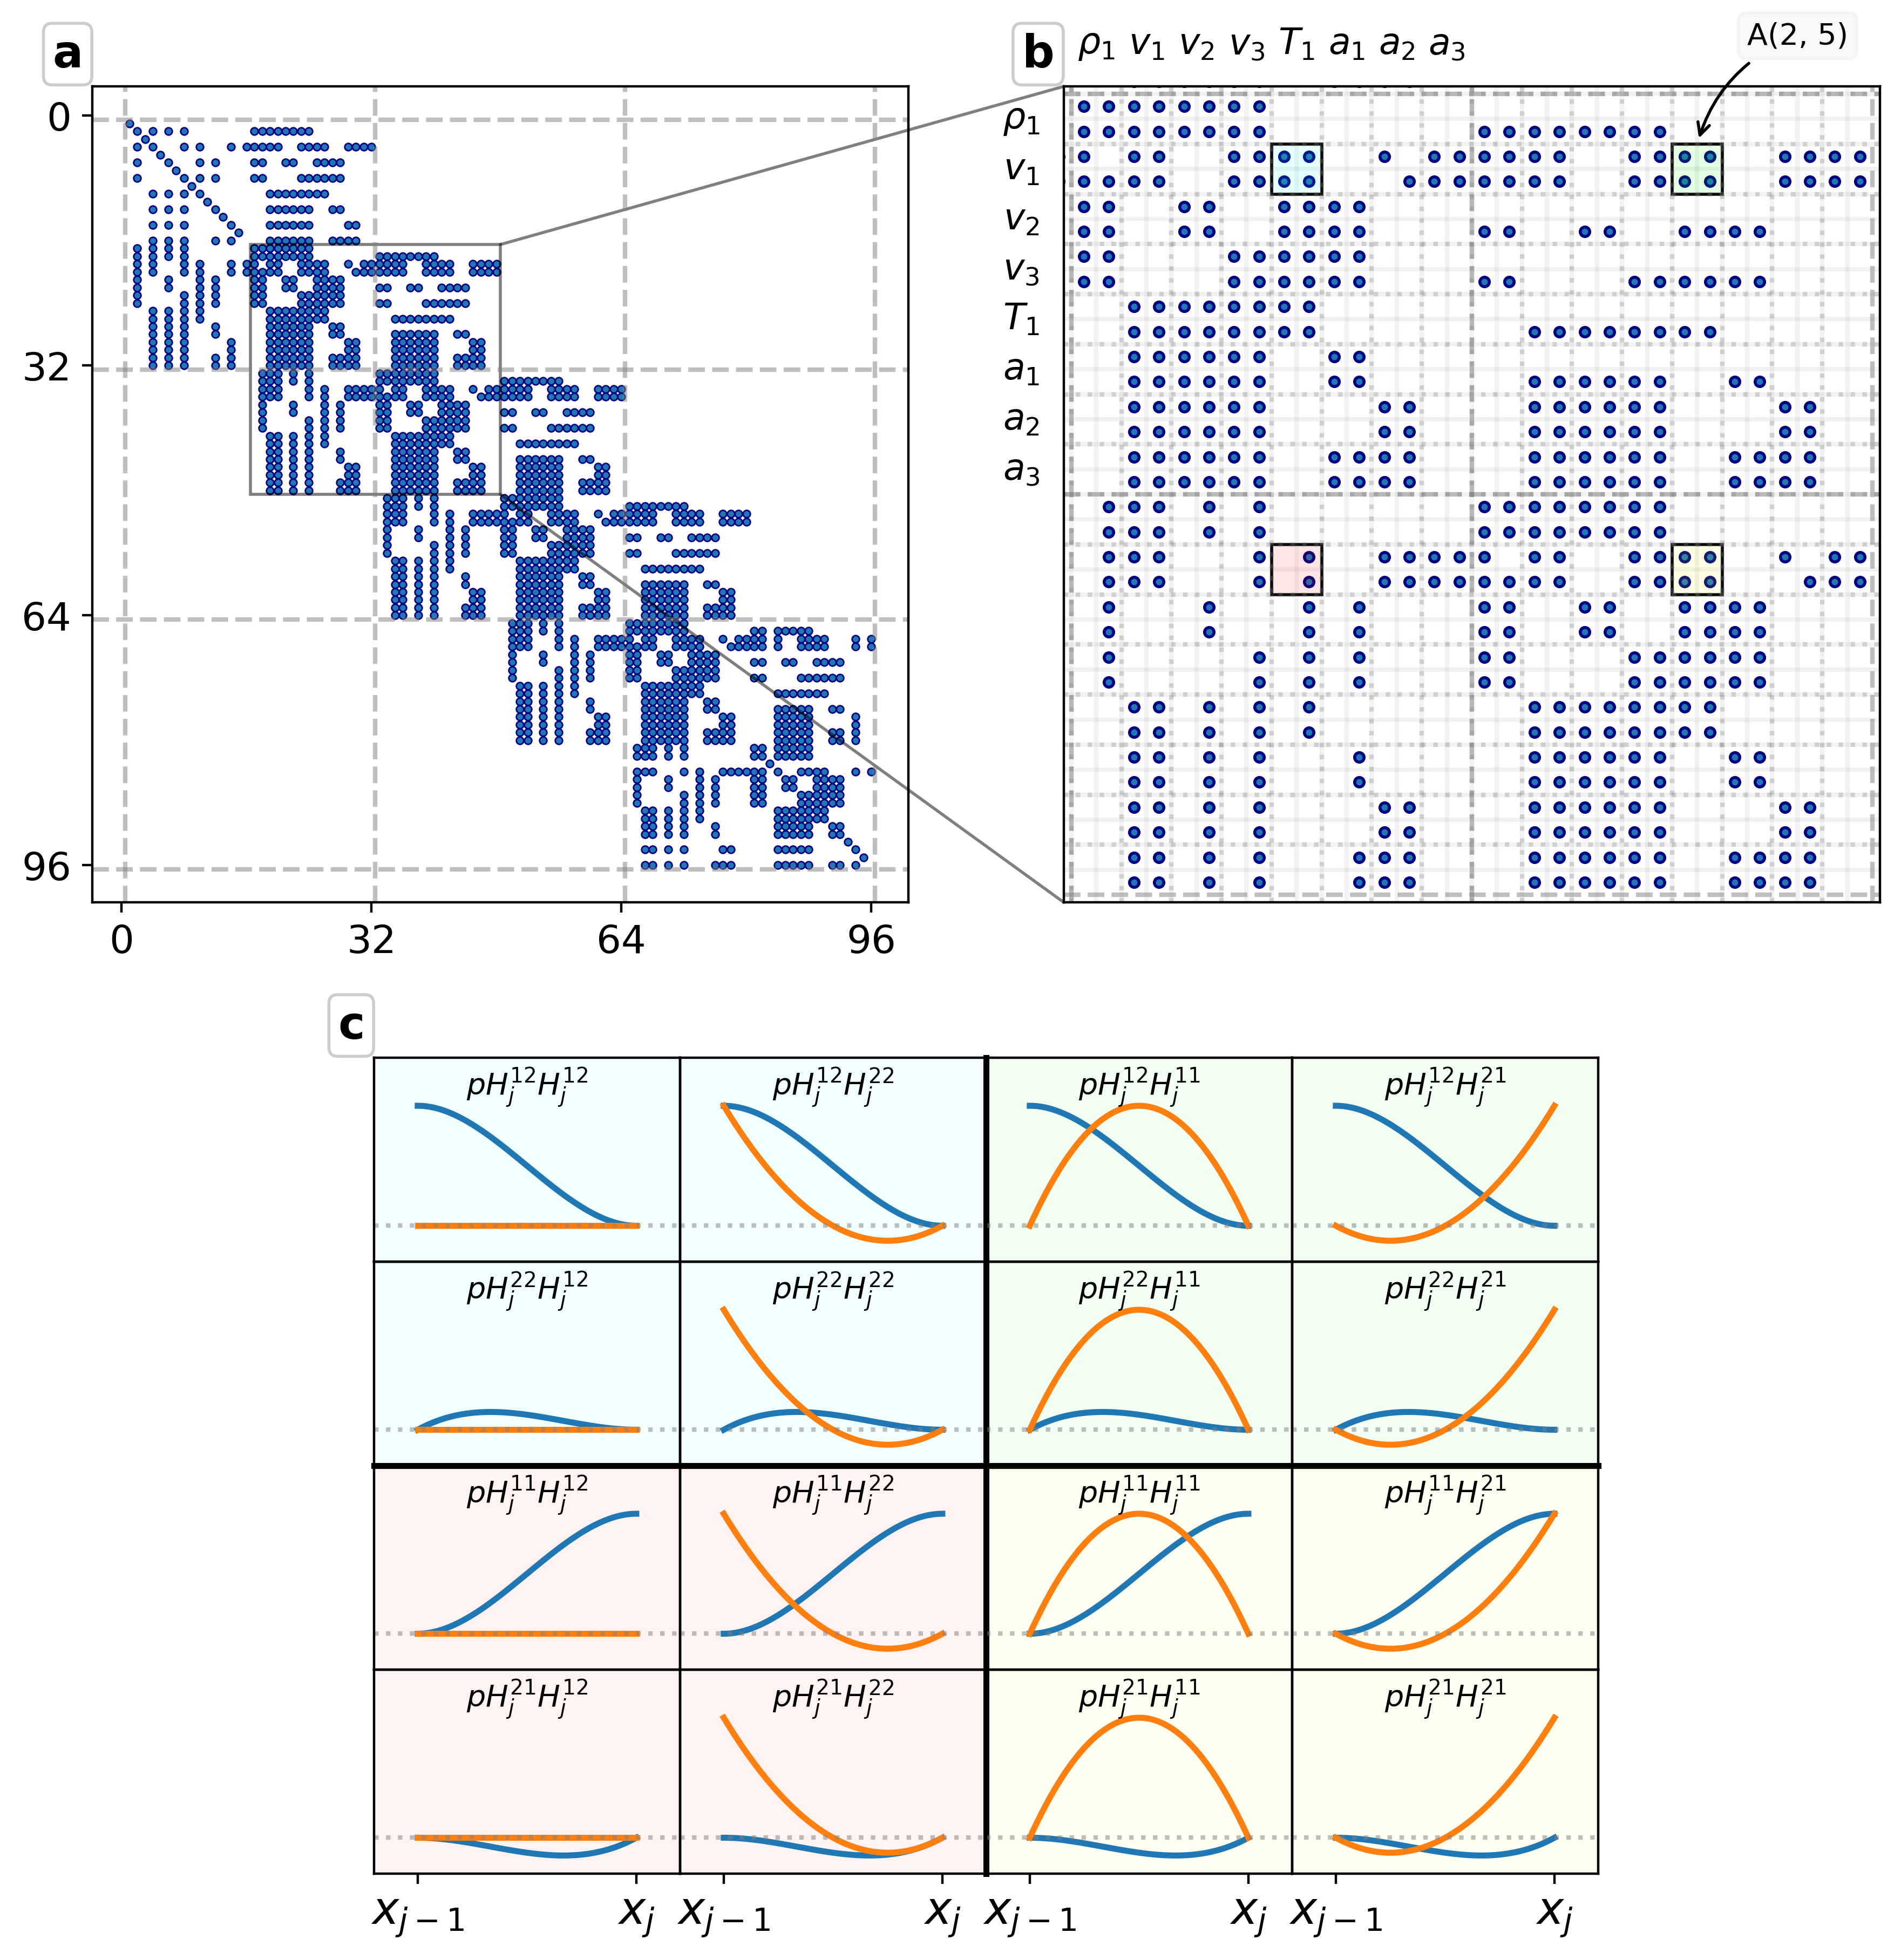
\includegraphics[width=\textwidth]{matrix_assembly.png}
  \caption{
    General assembly and structure of the finite element (complex) $\amat$ matrix. Panel \textbf{a}: example of a full matrix for six grid points, showing the block-tridiagonal structure where dots represent nonzero values. Panel \textbf{b} zooms in on one quadblock, showing the dependence of the different subblock positions with respect to the variables. The $2 \times 2$ blocks corresponding to (cubic, quadratic) element $(2, 5)$ are highlighted.
    Panel \textbf{c}: $2 \times 2$ block assembly for a general regular (cubic, quadratic) matrix element. Cubic elements are shown in blue, quadratic ones in orange. The dotted gray line denotes zero.
  }
  \label{fig: matrix_assembly}
\end{figure}

The term $pH_j^{\alpha\beta}H_j^{\alpha\beta}$ at the top of every subpanel on Panel c denotes which combination of the basis functions should be used, where $p$ stands for the integral coefficients. The exponent $\alpha\beta$ refers to the expressions for the basis functions, where $\alpha = 1$ stands for $Q_j^1$ or $C_j^1$, that is, Equations \eqref{eq: basisfunction_Q1} and \eqref{eq: basisfunction_C1}; while $\alpha = 2$ stands for $Q_j^2$ or $C_j^2$, hence Equations \eqref{eq: basisfunction_Q2} and \eqref{eq: basisfunction_C2}, depending on the variable under consideration (quadratic or cubic). The parameter $\beta$ stands for which part of the basis function should be taken: $\beta = 1$ means the first equation in cases, while $\beta = 2$ means the second one. As an example, we can look at $H_j^{12}H_j^{21}$: because $\amat(2, 5)$ represents a cubic and quadratic variable, this translates into $C_j^{12}Q_j^{21}$. For the cubic part, we therefore take the second equation of $C_j^1$, corresponding to $x_j \leq x \leq x_{j + 1}$. The quadratic part on the other hand is given by $Q_j^{21}$, which means that we take the first equation of $Q_j^2$, corresponding to $x_{j-1} \leq x \leq x_j$. This process is repeated for all matrix elements.

{\legolas} implements ``matrix splitting'', which means that every physical contribution is treated as a separate matrix. This is mainly done for numerical reasons: the code will simply avoid calculating matrix elements corresponding to physical terms that were disabled, thereby avoiding unnecessary calculations. As every physical contribution has its own matrix, the eigenvalue problem can be written as
\begin{equation}
	\omega \Bigl[
	\underbrace{\bmat}_{\substack{\text{\tiny regular} \\ \text{\tiny terms}}}
	+ \underbrace{\bmathall}_{\substack{\text{\tiny Hall} \\ \text{\tiny terms}}}
	\Bigr]\statevec
	= \Bigl[
		\underbrace{\amat}_{\substack{\text{\tiny regular} \\ \text{\tiny terms}}}
		+ \underbrace{\flowmat}_{\substack{\text{\tiny flow} \\ \text{\tiny terms}}}
		+ \underbrace{\etamat}_{\substack{\text{\tiny resistive} \\ \text{\tiny terms}}}
		+ \underbrace{\viscmat}_{\substack{\text{\tiny viscous} \\ \text{\tiny terms}}}
		+ \underbrace{\coolmat}_{\substack{\text{\tiny cooling} \\ \text{\tiny terms}}}
		+ \underbrace{\condmat}_{\substack{\text{\tiny conductive} \\ \text{\tiny terms}}}
		+ \underbrace{\hallmat}_{\substack{\text{\tiny Hall} \\ \text{\tiny terms}}}
	\Bigr]\statevec,
\end{equation}
but for all intents and purposes we will simply call the left- and right-hand side of this equation the $\bmat$ and $\amat$-matrices, respectively.


\subsubsection{Boundary conditions}
The system of differential Equations \eqref{eq: full_continuity}--\eqref{eq: full_induction3} still has to be complemented by a set of appropriate boundary conditions on both sides of the domain. For a Cartesian geometry, we look at a domain enclosed by two conducting walls. Clearly, the velocity component perpendicular to the walls has to be zero because there cannot be any propagation into a solid boundary. Mathematically, this translates into $\bv \cdot \unit{n} = 0$, where $\unit{n}$ represents the normal vector to the wall. Following the same reasoning, we also require that $\bb \cdot \unit{n} = 0$, so in terms of a vector potential, this implies $\unit{n} \times \ba = 0$. Hence, applying this to the set of linearised equations means that for the Cartesian case $v_1, a_2$, and $a_3$, all have to be zero on the boundaries. Furthermore, because we are dealing with a perfectly conducting wall, one has to take care when thermal conduction is included. In that case, the rigid wall directly influences the temperature because it acts as an energy reservoir essentially eliminating the temperature perturbation. Hence, if and only if perpendicular thermal conduction is taken into account, we have to supplement the boundary conditions by an additional conditions $T_1 = 0$ at the boundary. In theory there is a second possibility, which is treating the wall as a perfect insulator instead of a perfect conductor. In that case, there is no heat flux, which translates to the boundary condition $T_1' = 0$ instead of $T_1 = 0$. For now, we only consider the latter condition, that is, the one corresponding to a perfectly conducting wall.

In cylindrical geometry, we have the exact same boundary conditions as for the Cartesian case at the outer wall $r = R$, or at the outer edge of the accretion disk at $R$. The same is true at the inner disk edge, but for a flux tube extending to $r = 0$ we have to take the regularity conditions into account when treating the cylinder axis $r = 0$, which comes down to the fact that $r v_r$ should go to zero when approaching $r = 0$. Looking back at the transformations \eqref{eq: transformation} we applied, it follows that this condition is equivalent to $\widetilde{v_1} = 0$. Analogously, the same holds true for $a_2$ and $a_3$ such that these conditions are identical to the ones we applied for the Cartesian case, which is quite convenient implementation-wise. We again have to consider an additional condition if perpendicular thermal conduction is taken into account, because then $r T_1 = 0$ should also hold on the cylinder axis, which, similar to $v_1$, translates into $\widetilde{T_1} = 0$ at $r = 0$.

In the case of confinement by a perfectly conducting wall, we thus have straightforward boundary conditions, that is, $v_1 = 0, a_2 = 0, a_3 = 0$, and $T_1 = 0$ for both the Cartesian and cylindrical geometries on both sides (dropping the tildes). The latter boundary condition should only be taken into account if and only if perpendicular thermal conduction is included. These conditions are called \emph{essential boundary conditions}, meaning they \emph{have} to be satisfied by the system and should thus be explicitly handled.

\paragraph{Natural boundary conditions}
The integration by parts resulting from the weak Galerkin formulation gives rise to additional surface terms, which should also be evaluated at the boundaries. These kinds of conditions are called \emph{natural boundary conditions}, as they emerge in a natural way by reducing second-order derivatives to first-order derivatives when rewriting the eigenvalue problem. For simplicity we consider $B_{01} = v_{01} = 0$. In this case the additional surface terms for the momentum equation can be written as

\begin{equation} \label{eq: natural_boundary_v1}
  \begin{aligned}
    S_{v_1} &= \left[
      T_0 \hj{2}\hk{1}
      + \rho_0\hj{2}\hk{5}
      - \eps \Gmin \hj{2}\hk{6}
      + B_{03}\hj{2}\dhk{7}
      - \eps B_{02}\hj{2}\dhk{8}
    \right]_{\partial \Omega} \\
    &= v_1 \Bigl[
      T_0 \rho_1
      + \rho_0 T_1
      - \eps \Gmin a_1
      + B_{03}a_2'
      - \eps B_{02}a_3'
    \Bigr]_{\partial \Omega},
  \end{aligned}
\end{equation}
where the number in the superscript on $h_{j/k}$ denotes the index of the variable in the state vector $\statevec$.
The subscript $\partial \Omega$ means that these terms should be evaluated at the left or inner edge, as well as at the right or outer edge. In a similar manner, the surface terms for the energy and induction equations are given by
\begin{equation} \label{eq: natural_boundary_T1}
  \begin{aligned}
    S_{T_1} &= \icomplex \gmone T_1\Biggl[
      T_0'\dkappaperpdrho \rho_1
      + \left(T_0'\dkappaperpdT - \frac{\eps'}{\eps}\skappaperp{0}\right)T_1
      + \skappaperp{0}T_1'
    \Biggr. \\
    &+ 2\left(\eta_0 k_3 (\eps B_{02})' - \eta_0 k_2 B_{03}' - \eps T_0' \Gmin \dkappaperpdB\right)a_1 \\
    &+ 2\left(T_0' B_{03} \dkappaperpdB + \eta_0 B_{03}'\right)a_2'
     - 2\left(\eps B_{02}T_0'\dkappaperpdB + \eta_0 (\eps B_{02})'\right)a_3'
    \Biggr],
  \end{aligned}
\end{equation}

\begin{equation} \label{eq: natural_boundary_a2}
  S_{a_2} = \icomplex \eta_0 a_2 \bigl(a_2' - k_2 a_1\bigr),
\end{equation}

\begin{equation} \label{eq: natural_boundary_a3}
  S_{a_3} = \icomplex \eta_0 \eps a_3 \bigl(a_3' - k_3 a_1\bigr),
\end{equation}

which should all be evaluated at the boundaries. For the case of a solid wall, we see that the natural boundary conditions simplify considerably, because if $v_1, a_2$, and $a_3$ are all zero at the wall, then $S_{v_1}, S_{a_2}$ and $S_{a_3}$ are also zero and can be omitted. The natural boundary condition on $T_1$ is only relevant if resistivity or perpendicular thermal conduction is included. However, in the case of the latter, the additional essential boundary condition requires that $T_1 = 0$, in which case $S_{T_1}$ drops out as well. The only combination in which the surface terms for the energy equation are nonzero is when resistivity is included but perpendicular thermal conduction is omitted. In that case, the resistive heating terms should be included in the calculation, which is done by adding the appropriate terms to the matrix elements $\amat(5, 6)$, $\amat(5, 7)$ and $\amat(5, 8)$.

Currently, only fixed wall boundary conditions are implemented in {\legolas}. However, the surface terms described here can be used to impose other types of boundary conditions as well. In the case of a plasma-vacuum-wall transition, we have, for example, Bessel functions at the outer boundary of a cylindrical geometry \citep{book_roberts}, which encode the analytic vacuum solution for the electromagnetic field in the outer vacuum region. These expressions can then be used to rewrite the surface terms \eqref{eq: natural_boundary_v1}--\eqref{eq: natural_boundary_a3} in an appropriate way such that they can be added to their respective subblock positions in the matrix. This is one of the planned extensions to be included in future versions of {\legolas}.

\paragraph{Essential boundary condition}
The essential boundary conditions as described earlier have to be implemented explicitly. This is done by omitting the relevant basis functions that do not satisfy the boundary conditions on the edges. Consider as an example the variable $v_1$, which is associated with a cubic basis function. From Figure \ref{fig: basisfunctions}, we see that the only cubic element that is nonzero at the left boundary is $C_j^{12}$, which implies that the matrix elements where it appears should be zeroed out. Looking back at how the quadblock is composed in Figure \ref{fig: matrix_assembly}, the boundary condition $v_1 = 0$ corresponds to forcing the odd rows and columns of the $v_1$ contribution to zero, for subblocks $1, 2,$ and $3$ on the left boundary (that is, the first node $j$) because these correspond to the $2 \times 2$ blocks in blue, green and red on the right panel. Similarly, on the right side (viz. the last node $j$), only $C_j^{11}$ is nonzero, which implies that the odd rows and columns of subblocks $2, 3,$ and $4$ have to be zeroed out (corresponding to green, red, and yellow). Extending this reasoning to the essential boundary condition on $T_1$, we see that in this case the even rows and columns should be handled because $T_1$ is associated with a quadratic element. This is done for both matrices.

Of course, ``just'' zeroing out rows and columns in a matrix has the unpleasant side effect that the matrices become singular. For the $\amat$-matrix, this is not necessarily a problem; however, the $\bmat$ matrix is not allowed to be singular because it is inverted when solving the general eigenvalue problem using the QR-algorithm. Therefore, we introduce a one on $\bmat$'s diagonal at the location that was zeroed out, and an element $\delta$ on $\amat$'s diagonal. The effect of this is that one essentially ``forces'' the boundary condition, because this implies that $\delta x_j^i = \omega x_j^i$. By extension, if $\delta$ is taken to be a large number (we take $\delta = 10^{20}$), this means that $x_j^i = 0$ which corresponds to the essential boundary we want to impose. The only side effect of this approach is that it introduces eigenvalues equal to $\delta$. However, because $\delta$ is taken to be large, these will not influence the spectrum in any way, and they can be easily filtered out during postprocessing. This method thus provides a relatively easy and straightforward way to impose Dirichlet boundary conditions at the edges. The imposed boundary conditions are noticeable on Panel a of Figure \ref{fig: matrix_assembly}, especially for the first node. The odd rows and columns that were zeroed out can clearly be seen, together with the elements introduced on the main diagonal.



% \subsubsection{Assembly of the eigenfunctions}
% \subsubsection{Derived eigenfunction quantities}


\cleardoublepage
